\documentclass[fancy, masters]{byuthesis}
% Class options are simple/fancy and masters/phd.
% Leave options blank for defaults.
% Defaults are simple for document style, and masters for degree type.


%%%%%%%%%%%%%%%%%%%%%%%%%%%%%%%
% Custom options and packages %
%%%%%%%%%%%%%%%%%%%%%%%%%%%%%%%
% Define path to figure files
\graphicspath{{figures/}}

% Define sequences of Latin text to fill space in example documents
% (not needed for your thesis -- delete or comment out if you'd like)
\usepackage{blindtext}


%%%%%%%%%%%%%%%%%%%%%%%%%%%%%%
% Define title page elements %
%%%%%%%%%%%%%%%%%%%%%%%%%%%%%%
% Thesis title for required BYU title page
\title{Forecasting Ride-hailing across\\
\hspace*{0.333em}Multiple Model Frameworks}

% On the custom title page, use the same title, but format as you like
\customtitle{Forecasting Ride-hailing across\\
\hspace*{0.333em}Multiple Model Frameworks}

% Your name goes here:
\author{Christopher Day}

% This is the date of graduation
\date{April 2021}

% If your degree is not a PhD or MS, then you can overwrite the degree using
\degree{Master of Science}

% Your department
\department{Department of Civil and Construction Engineering}

% The names of your committee members
\committeechair{Gregory S. Macfarlane}
  \committeemember{Grant G. Schultz}
  \committeemember{Gustavious P. Williams}

% Include any keywords you would like for your thesis/dissertation
\keywords{activity-based model, multi-agent simulation, novel transport modes, ActivitySim, BEAM}


%%%%%%%%%%%%%%%%%%%%%%%%%%%%%%%%%%
% ---Bibliography source file--- %
%%%%%%%%%%%%%%%%%%%%%%%%%%%%%%%%%%
	\usepackage{algorithm}
\usepackage{algpseudocode}
\usepackage{dsfont}
\usepackage{pdflscape}
\usepackage{graphicx}
\usepackage{mathtools}
\usepackage{eqparbox}
\usepackage{makecell}
	\usepackage{booktabs}
\usepackage{longtable}
\usepackage{array}
\usepackage{multirow}
\usepackage{wrapfig}
\usepackage{float}
\usepackage{colortbl}
\usepackage{pdflscape}
\usepackage{tabu}
\usepackage{threeparttable}
\usepackage{threeparttablex}
\usepackage[normalem]{ulem}
\usepackage{makecell}
\usepackage{xcolor}


%%%%%%%%%%%%%%%%%%%%%%%%%%%%%%%%%%
% ---Bibliography source file--- %
%%%%%%%%%%%%%%%%%%%%%%%%%%%%%%%%%%
%  Default is references.bib
\bibliography{}

\newlength{\cslhangindent}
\setlength{\cslhangindent}{1.5em}
\newlength{\csllabelwidth}
\setlength{\csllabelwidth}{3em}
\newlength{\cslentryspacingunit} % times entry-spacing
\setlength{\cslentryspacingunit}{\parskip}
% for Pandoc 2.8 to 2.10.1
\newenvironment{cslreferences}%
  {}%
  {\par}
% For Pandoc 2.11+
\newenvironment{CSLReferences}[2] % #1 hanging-ident, #2 entry spacing
 {% don't indent paragraphs
  \setlength{\parindent}{0pt}
  % turn on hanging indent if param 1 is 1
  \ifodd #1
  \let\oldpar\par
  \def\par{\hangindent=\cslhangindent\oldpar}
  \fi
  % set entry spacing
  \setlength{\parskip}{#2\cslentryspacingunit}
 }%
 {}
\usepackage{calc}
\newcommand{\CSLBlock}[1]{#1\hfill\break}
\newcommand{\CSLLeftMargin}[1]{\parbox[t]{\csllabelwidth}{#1}}
\newcommand{\CSLRightInline}[1]{\parbox[t]{\linewidth - \csllabelwidth}{#1}\break}
\newcommand{\CSLIndent}[1]{\hspace{\cslhangindent}#1}

\providecommand{\tightlist}{%
  \setlength{\itemsep}{0pt}\setlength{\parskip}{0pt}}

%%%%%%%%%%%%%%%%%%%%%%%%%%
% --- Begin Document --- %
%%%%%%%%%%%%%%%%%%%%%%%%%%
\begin{document}


%%%%%%%%%%%%%%%%%%%%%%%%%%%%%%%%%%%%%%%%%%%%%%%%%%%%%%%
% --- Front matter (probably don't need to change)--- %
%%%%%%%%%%%%%%%%%%%%%%%%%%%%%%%%%%%%%%%%%%%%%%%%%%%%%%%
	\frontmatter

	\titlepage
	\clearpage

	\customtitlepage
	\clearpage


    \begin{abstract}
  The advent of on-demand transport modes such as ride-hailing and microtransit has challenged forecasters to develop new methods of forecasting the use and impacts of such modes. In particular, there is some professional disagreement about the relative role of activity-based transportation behavior models --- which have detailed understanding of the person making a trip and its purpose --- and multi-agent demand simulations which may have a better understanding of the availability and service characteristics of on-demand services. A particular question surrounds how the relative strengths of these two approaches might be successfully paired in practice. Using daily plans generated by the activity-based model ActivitySim as inputs to the BEAM multi-agent simulation, we construct nine different methodological combinations by allowing the choice to use a pooled ride-hail service in ActivitySim, BEAM, or both. Within each combination, we estimate ride-hailing ridership and level of service measures. The results suggest that a multi-agent simulation may overstate the demand interest relative to an activity-based model, but there may be opportunities to implement feedback loops to strengthen the forecasting power.
  \end{abstract}
  	\clearpage


    \begin{acknowledgments}
  I would first like to acknowledge my advisor and friend, Dr.~Gregory Macfarlane, for teaching me everything I know. Without you, this thesis and my future career would be boring and stupid. I found a work to love and enjoy while researching under your supervision, and for that I will forever be grateful. I express gratitude as well to Dr.~Shultz and Dr.~Williams for being on my advisory committe and helping me finish my thesis. I would also like to acknowledge the United States Department of Transportation (USDOT) for funding my research. Thank you to the members of the T-SCORE center, especially Dr.~Gregory Erhardt, Jawad Hoque, and Vedant Goyal for their friendship and help with tackling BEAM. A special shoutout to Nate Lant and Hayden Atchley for working on ActivitySim and BEAM even when we had no idea what we were doing. Together, we got this thing done. I am enormously grateful as well to Zachary Needell at Lawrence Berkeley National Laboratory for working with the T-SCORE team and I in our efforts to tame BEAM. Without you, none of this would have been possible. An additional thanks to Wasatch Front Regional Council, especially Chad Worthen, for sharing data and working with our group. I express sincere gratitude for my family members and their patience and support as I conducted this research. Especially, thank you to my wife Megan, because without her I would probably be dead. She convinced me to apply for this research position, held down the fort at home, let me work every Saturday for 3 years, and was patient with me everytime I went insane staring at my computer screeen. I appretiate you all. Finally, thank you to the BYU tennis courts and Kevin Lunt, because tennis is the key to happiness.
  \end{acknowledgments}
  	\clearpage

	\tableofcontents*
	\clearpage

	\listoffigures
	\clearpage

	\listoftables
	\clearpage

	\nomenclature{$c$}{Speed of light in a vacuum inertial frame}
\nomenclature{$h$}{Planck constant}
\nomenclature{$\mathit{Re}$}{Reynolds number}
\nomenclature{$\mathbf{x}$}{State vector}
\nomenclature{$\alpha$}{Angle of attack}
\nomenclature{$\beta$}{Sideslip angle}
\nomenclature{$\gamma$}{Climb angle}
\nomenclature{$p$}{Roll rate}
\nomenclature{$q$}{Pitch rate}
\nomenclature{$r$}{Yaw rate}
\nomenclature{$P$}{Covariance matrix}

\printnomenclature
	\clearpage

%%%%%%%%%%%%%%%%%%%%%
% --- Main Body --- %
%%%%%%%%%%%%%%%%%%%%%
	\mainmatter

\hypertarget{intro}{%
\chapter{Introduction}\label{intro}}

\hypertarget{problem-statement}{%
\section{Problem Statement}\label{problem-statement}}

On-demand transit modes, such as microtransit and ride-hailing, can make private car-centric societies more sustainable. They have the potential to exhaust less vehicular emissions, decrease roadway congestion, increase health, increase public transit usage in some cases, and be economically viable Chen et al. (2021). As urban centers attempt to shift from a private car-centric environment to a multi-modal system, forecasters are challenged with modeling accurate ridership and level of service values. Since ride-haling is already heavily involved in today's transportation system, estimating the uptake of ride-hailing usage and understanding the service capabilities of ride-hailing is critical to a sustainable future.

Unfortunately, forecasting the ridership and level of service of ride-hailing and other novel modes is a challenging feat with no clear methodological approach. Ride-hailing vehicles behave differently than regular car modes and given their unique nature, understanding their behavior and service capabilities is particularly challenging (e.g., Kang et al. (2021), Y. Li et al. (2020), X. Dong (2020), Dean \& Kockelman (2021)). In addition, the ridership of bike share, an affordable and sustainable bike rent program, has been modeled many times each with a different methodology (e.g., Hyland et al. (2018), Biehl et al. (2019), Cho \& Shin (2022), Li \& Kamargianni (2018), Welch et al. (2020), Zhou et al. (2019), Song et al. (2019)). Similarly, forecasters have struggled to find the best technique for estimating the ridership of e-scooters (public electric scooters) and in what locations they would be most effective (e.g, Zuniga-Garcia et al. (2022), Tuli et al. (2021), Zhang et al. (2021), M. Lee et al. (2021), H. Lee et al. (2021), Hosseinzadeh et al. (2021)). Overall, various attempts have been made to model the ridership and level of service of ride-hailing and other novel modes.

Many different modeling software exists with the purpose of better understanding the travel behavior of ride-hailing vehicles and other novel modes. For example, some forecasters model the service capabilities of novel transport modes with activity-based models, which use daily activity patterns as the central tool to model an individual's travel behavior (e.g., Xu et al. (2019), Muhammad et al. (2019), Macfarlane et al. (2021)). Other forecasters use multi-agent simulation, which focuses on modeling the interactions between different agents, to understand the level of service of transport technologies (e.g., Shimizu et al. (2013), Sánchez et al. (2019), Hörl, Ruch, et al. (2019)). Some chose a simpler approach, spatial analysis and geography data, to model modal behavior and level of service (e.g., Hyland et al. (2018), Cho \& Shin (2022), Hosseinzadeh et al. (2021)). Forecasters have even attempted to use machine learning techniques (e.g., Zhou et al. (2019)). Among these, and the other strategies that exist, some profession disagreement exists as to which approach would best serve forecasters in their efforts to model the ridership and level of service of ride-hailing to create sustainable city centers. In particular, a lack of understanding exists as to if the relative strengths of an activity-based model and multi-agent simulation could be paired together successfully to model the uptake of on-demand services.

\hypertarget{purpose-of-research}{%
\section{Purpose of Research}\label{purpose-of-research}}

In this paper, we develop a series of experiments to understand the relative importance of a paired activity-based model and multi-agent simulation in forecasting the uptake of ride-hailing. We do this by examining the ridership and level of service of ride-hailing generated by different activity-based model and multi-agent simulation mode choice combinations. Specifically, we use the daily activity plans generated by ActivitySim as inputs to the multi-agent simulation BEAM to establish 9 different mode choice combinations. For each methodological combination, we estimate ride-hailing ridership and level of service outputs for a Salt Lake City, Utah case study region.

\hypertarget{lit}{%
\chapter{Literature Review}\label{lit}}

As discussed in Section \ref{intro}, forecasters have attempted to model the behavior and level of service of ride-hailing and other novel modes in a variety of ways. Since there is some disagreement as to which strategy best forecasts ridership and behavior, the following literature review outlines the pros and cons of using spatial analysis, activity-based models, multi-agent simulation, and paired modeling approaches to model the use and impacts of ride-hailing. Since the behavior of other novel modes is similar to that of ride-hailing, we include references to research completed for other novel modes as well.

\hypertarget{lit-simp}{%
\section{Statial Analysis and Ride-hailing}\label{lit-simp}}

The most prominent methodological approach to understanding ride-hailing service is through simple approaches like spatial, statistical, and empirical analyses. For example Correa et al. (2017) developed heatmaps using spatio-temporal data to analyze ride-hailing pickup locations. Marquet (2020) processed data and used statistical measures to estimate a connection between walkability index and ride-hailing usage. Y. Dong et al. (2018) conducted an empirical analysis to understand the unique travel patterns of ride-hailing vehicles. Many other research studies have used simple approaches to estimate the ridership and service of ride-hailing and other novel modes (e.i, Li et al. (2022), Hyland et al. (2018), Cho \& Shin (2022), Hosseinzadeh et al. (2021), Zhou et al. (2019), etc.). The upside to implementing such strategies is their simplicity. The downside, however, is that with their simplicity comes decreased flexibility. Simple spatial, statistical, and empirical methods oftentimes only answer one particular service related question. They are unable to accurately forecast the ridership, level of service, and other usage measures simultaneously whereas activity-based models and multi-agent simulations can.

\hypertarget{lit-abm}{%
\section{Activity-based Models and Ride-hailing}\label{lit-abm}}

Activity-based models are transportation behavior models that construct daily activity patterns for synthetic individuals from behavior choice models. To accurately represent the way people travel, activity-based models predict activity demand before travel demand (Philip et al., 2013). Activity-based models also use utility theory and logit based regression to estimate individual behavior (Bowman, 1998). These models were designed for which their primary advantage is strong individual behavioral representation. Representing individual behavior accurately is advantageous when trying to estimate ride-hailing services, like ridership, because it predicts who among the population is most likely to use a ride-hailing vehicle. In addition to representing behavior accurately, another advantage to using activity-based models is the modal consistency between trips on the same tour (e.g., Nayak \& Pandit (2022), Hasnine \& Nurul Habib (2021), Knapen et al. (2021), Gomes et al. (2021)). Individuals act similarly among trips of the same tour, and activity-based models account for this natural tendency by chaining trips of the same individual together. By maintaining modal consistency among individuals, ride-hailing usage is consistently distributed to the same trips and same individuals, further suggesting justifiable ride-hailing selection estimates.

Knowing the advantages that activity-based models provide, many forecasters use activity-based models to model the ridership and travel patterns of ride-hailing and other novel modes. For example, Nguyen et al. (2022) modeled one-way car-sharing services with an activity-based model because the modal consistency between trips allowed them to estimate vehicle usage. Xu et al. (2019) modeled privately-owned autonomous vehicles with an activity-based model as a way to better understand their impact on household travel patterns. Rafiq \& McNally (2022) used an activity-based approach to estimate the five most common tour structures of ride-hailing individuals. Many forecasters elect to use activity-based models to model ride-hailing and other modes because of the behavioral representation and modal consistency they provide.

Although there are advantages to using activity-based models to model ride-hailing, forecasters must consider the various weaknesses that exist when using activity-based models. One of the biggest shortfalls with most activity-based models is that travel times are averaged along travel links (e.g., RSG (2016), Mahmoudi et al. (2021)). For example, although Nguyen et al. (2022) used an activity-based models to model one-way car sharing, they noted that it used the Bureau of Public Roads (BPR) function to estimate travel time. The BPR function is a regression function that estimates average travel time based on arrival flows. When using the BPR function to estimate smaller time intervals though, it becomes inconsistent. For this reason, Nguyen et al. (2022) noted that it was more difficult to verify the service capabilities of the car-sharing modes. Activity-based models lack variability when modeling travel and wait times of ride-hailing and other novel vehicles. In addition, it can be difficult to model ride-hailing vehicle availability and passenger capacity limitations. Almost inversely, however, multi-agent simulation excels at estimating service capabilities but lacks in accurate behavioral representation.

\hypertarget{lit-mas}{%
\section{Multi-agent Simulation and Ride-hailing}\label{lit-mas}}

An alternative to activity-based models for forecasting ride-hailing level of service is multi-agent simulation. Multi-agent simulation models interactions between individual agents (e.g., Bazghandi (2012), Amblard et al. (2015), Siebers \& Aickelin (2008)). By forecasting the travel behavior on an individual level, multi-agent simulation provides a slew of travel behavior detail at the individual level. This means that wait time and travel time estimations vary between every agent. Forecasting level of service with unique travel time statistics will produce more realistic results. Along with modeling each individual closely, a multi-agent simulation keeps track of every ride-hailing vehicle as well. The complexity of the vehicular availability model along with individual travel behavior model allows multi-agent simulation to estimate exact, variable wait and travel times. For example, the model knows the exact ride-hailing vehicle availability and ride-hailing passenger capacity at every moment of the day. Therefore, capacity measures, like ride-hailing ridership and utilization, can be estimated realistically and with great precision at the individual level using multi-agent simulation.

Due to the advantages that multi-agent simulation provides, various forecasters have elected to use them to model the level of service for ride-hailing and other novel transport modes. For example, Kamel et al. (2019) chose to use a multi-agent simulation to model shared autonomous vehicles because decision-making was done on an individual level. This granularity helped the researchers understand how user preferences affected the modal split of shared autonomous vehicles. Hörl, Ruch, et al. (2019) also analyzed shared autonomous vehicles with a multi-agent simulation, mainly to take advantage of the detailed vehicular model. The model allowed forecasters to adjust fleet size and to optimize the way fleet vehicles behaved. By utilizing the advanced vehicular model, the researchers were able to estimate the overall system performance, wait times, and cost of various autonomous vehicle fleets. Similarly, Becker et al. (2020) used MATSim, an open source agent-based simulation used for large scale scenarios, to model the travel times and costs of different on-demand transit modes (ride-hailing, car-sharing, bike-sharing). The primary advantage of MATSIM is that it provides a ``dynamic demand response towards changes in service attributes such as travel times or costs'' (Becker et al., 2020). Many forecasters continue to analyze new transportation technologies with multi-agent simulation because its inherit advantages are helpful to understanding service capabilities.

Although multi-agent simulation excels at estimating the level of service of ride-hailing vehicles at fine detail, various pitfalls do exists. For example, Ciari et al. (2016) summarizes a multitude of research done to understand demand for car-sharing with the multi-agent simulation model MATSim. In this research, they note that although multi-agent simulation provides an extensive level of detail, it does not necessarily equate to real world accuracy. Because of the complexity of the multi-agent simulation structure, it remains very difficult to accurately portray individual behavior choices. The structure of the activity-based choice model allows strong individual behavioral representation, whereas the complexity of the multi-agent simulation causes many individual choices to be inaccurate and unreasonable. Similarly, where the activity-based model may excel at more realistic mode choice selections among trips of the same tour, some multi-agent simulation struggle. For example, Figure\ref{fig:fig-mode-compare} provides a visual example of mode choice shortcoming present in some multi-agent simulations. As seen in Figure \ref{fig:fig-mode-compare}, all trips of the same tour for the activity-based model are based on the selected tour mode. (A tour mode represents the primary mode any particular agent selects to use on a sequence of trips starting and ending at the home location.) This allows users to switch from one mode to another between trips, as long as they are compatible. On the other hand, the simulation model may only undergo mode choice selection on the first trip of the tour, and be trapped into using that same mode on future trips. (Footnote: This is not true for all simulation models, but is true for the multi-agent simulation model used in this research project (BEAM).) This results in less realistic travel behavior. The last inherit weakness of multi-agent simulation is that it is computationally heavy; requiring abundant time and resources. Overall it is clear to see that where the multi-agent simulation lacks in forecasting ride-hailing services the activity-based model excels, and vice versa, and so the combination of using both strategies could prove effective.

\begin{figure}

{\centering 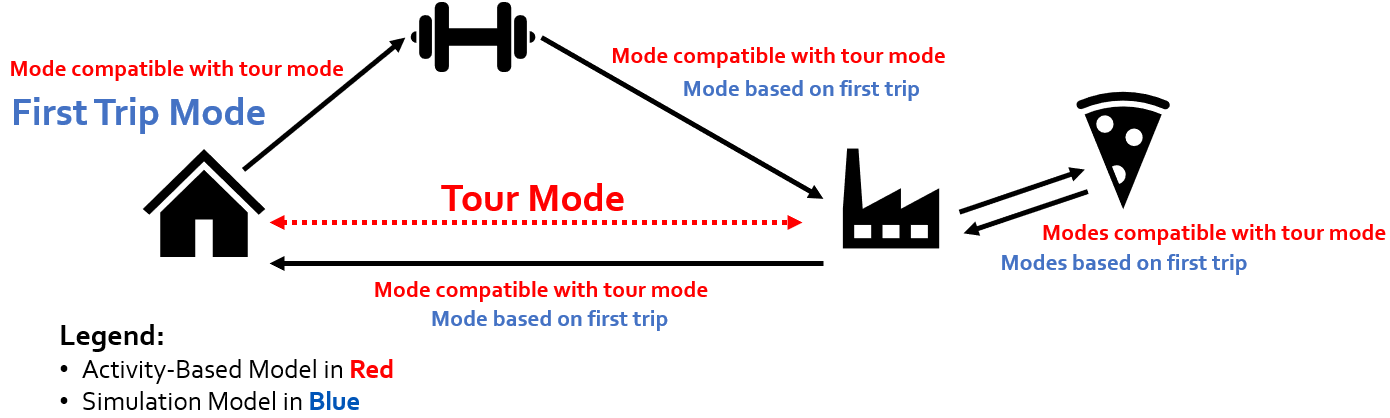
\includegraphics[width=1\linewidth]{pics/abm-mas-compare} 

}

\caption{Mode choice in activity-based models and multi-agent simulation.}\label{fig:fig-mode-compare}
\end{figure}

\hypertarget{limited-attempts-to-pair-two-disparate-modeling-approaches}{%
\section{Limited Attempts to Pair Two Disparate Modeling Approaches}\label{limited-attempts-to-pair-two-disparate-modeling-approaches}}

The varying strengths and weaknesses within both activity-based models and multi-agent simulation point to possibly using both approaches to understand ride-hailing ridership and level of service. Yet few forecasters have attempted to reconcile or pair these two disparate approaches in order to better understand the behavior of ride-hailing and other novel modes. However, one example of reconciling the traditional approaches is with the system MITO Zwick et al. (2021). MITO stands for Microsimulation Transport Orchestrator, and its primary purpose is to overcome the limitations of the traditional trip-based model while being easier to implement than the traditional activity-based model. Like a multi-agent simulation, MITO simulates each agent individually. MITO also includes a simplified activity schedule builder, allows forecasters to add attributes, allows agent tracing, and is not as computationally heavy as traditional multi-agent simulations (Moeckel et al., 2020). Zwick et al. (2021) used MITO to estimate travel demand and MATSim to simulate that demand. By pairing together MITO and MATSim, the researchers were able to gather service criteria for pooled on-demand ride-hailing vehicles at a detailed level, while also maintaining the behavioral integrity of each agent.

Another example of pairing together two disparate modeling approaches involves discrete choice and MATSIM. Since MATSim implements a feedback loop to determine mode choice instead of using a discrete choice model, some researches have attempted to pair together a discrete mode choice model with MATSim in attempt to shorten the number of iterations needed to be run. For example, Hörl, Balać, et al. (2019) discovered that by using a discrete choice model within MATSim, no irrelevant mode choice decisions were made. This indeed, lead to less iterations being run while enhancing the realistic nature of the mode choice selection. However, although initial modal decisions were more accurate than the default MATSim model, the discrete choice model added a layer of complexity. The need for more accurate and useful data gave the model runners less freedom.

Overall, these few examples show that by pairing together multiple model frameworks the strengths of each model is utilized. To the authors knowledge, however, no previous literature exists on pairing together an activity-based model and a multi-agent simulation for the purpose of modeling ride-hailing ridership and level of service. By using an activity-based model we can take advantage of the strong individual behavior representation and realistic mode choice decisions. By using a multi-agent simulation we can take advantage of the vaste individual travel behavior detail and the advanced vehicular availability model. We therefore hypothesize that with a joint activity-based model and multi-agent simulation, we can utilize the advantages of both models to capture ride-hailing ridership and level of service measures. And so, the objective of this study is to better understand the significance of using a linked activity-based model and multi-agent simulation in forecasting the usage of ride-hailing modes.

intro: 502 + 99 = 601
lit: 95 + 170 + 479 + 710 + 493 = 1947
meth: 85 + 77 + 294 + 343 + 69 + 363 + 482 + 598 = 2311
results: 70 + 907 + 580 + 127 + 63 + 114 + 466 + 331 + 53 = 2711
discuss: 352 + 105

(so far; 8027)

results: 2k
discuss: 500
limit:500
conclude:500

TOtal: 2585

\hypertarget{methods}{%
\chapter{Methods}\label{methods}}

We developed a series of experiments to understand the relative importance of pairing an activity-based and multi-agent simulation in forecasting the uptake of ride-hailing. We performed these experiments using ActivitySim as the activity-based model and BEAM as the multi-agent simulation. We used the Salt Lake City, Utah region as a case study for our experiments. The following section outlines the methodology for which we were able to model ride-haling ridership and level of service with differing activity-based model and multi-agent simulation mode choice combinations.

\hypertarget{meth-asim}{%
\section{ActivitySim as the Activity-based Model}\label{meth-asim}}

ActivitySim is an activity-based simulator used to generate plans for millions of agents each with their own demographic attributes (ActivitySim, 2021a). Instead of independently modeling each trip, ActivitySim simulates each individual by calculating their daily travel diaries and schedules. Long term decisions are made first, and then shorter term decisions are calculated based on those long term decisions ({``ActivitySim,''} 2021b). Overall, ActivitySim is an advanced activity-based model with the same advantages and disadvantages described in Section \ref{lit-abm}.

\hypertarget{ride-hailing-in-activitysim}{%
\subsection{Ride-hailing in ActivitySim}\label{ride-hailing-in-activitysim}}

We chose ActivitySim as the activity-based model in this research because it is an open-source software with ride-hailing modal alternatives built into its framework. Specifically, the ride hail mode and the pooled ride hail mode fall under one of the four nested tiers of ActivitySim's nested logit model. This means that ride hail is a unique modal option not characterized by being an auto, non-motorized, or transit type mode. Figure \ref{fig:fig-asim-nest} displays the four tiers of the nested logit along with the modal alternatives of each tier (MTC, 2012). These modal alternatives represent the alternatives available in both ActivitySim's tour based and trip based mode choice model. When determining the mode to use on a trip, ActivitySim first calculates the tour mode and subsequently calculates the trip mode based on the tour mode selection (See Figure \ref{fig:fig-mode-compare}). Person attributes, path attributes, location attributes, tour purpose value, and more all play a role in calculating the mode choice decision.

\begin{figure}

{\centering 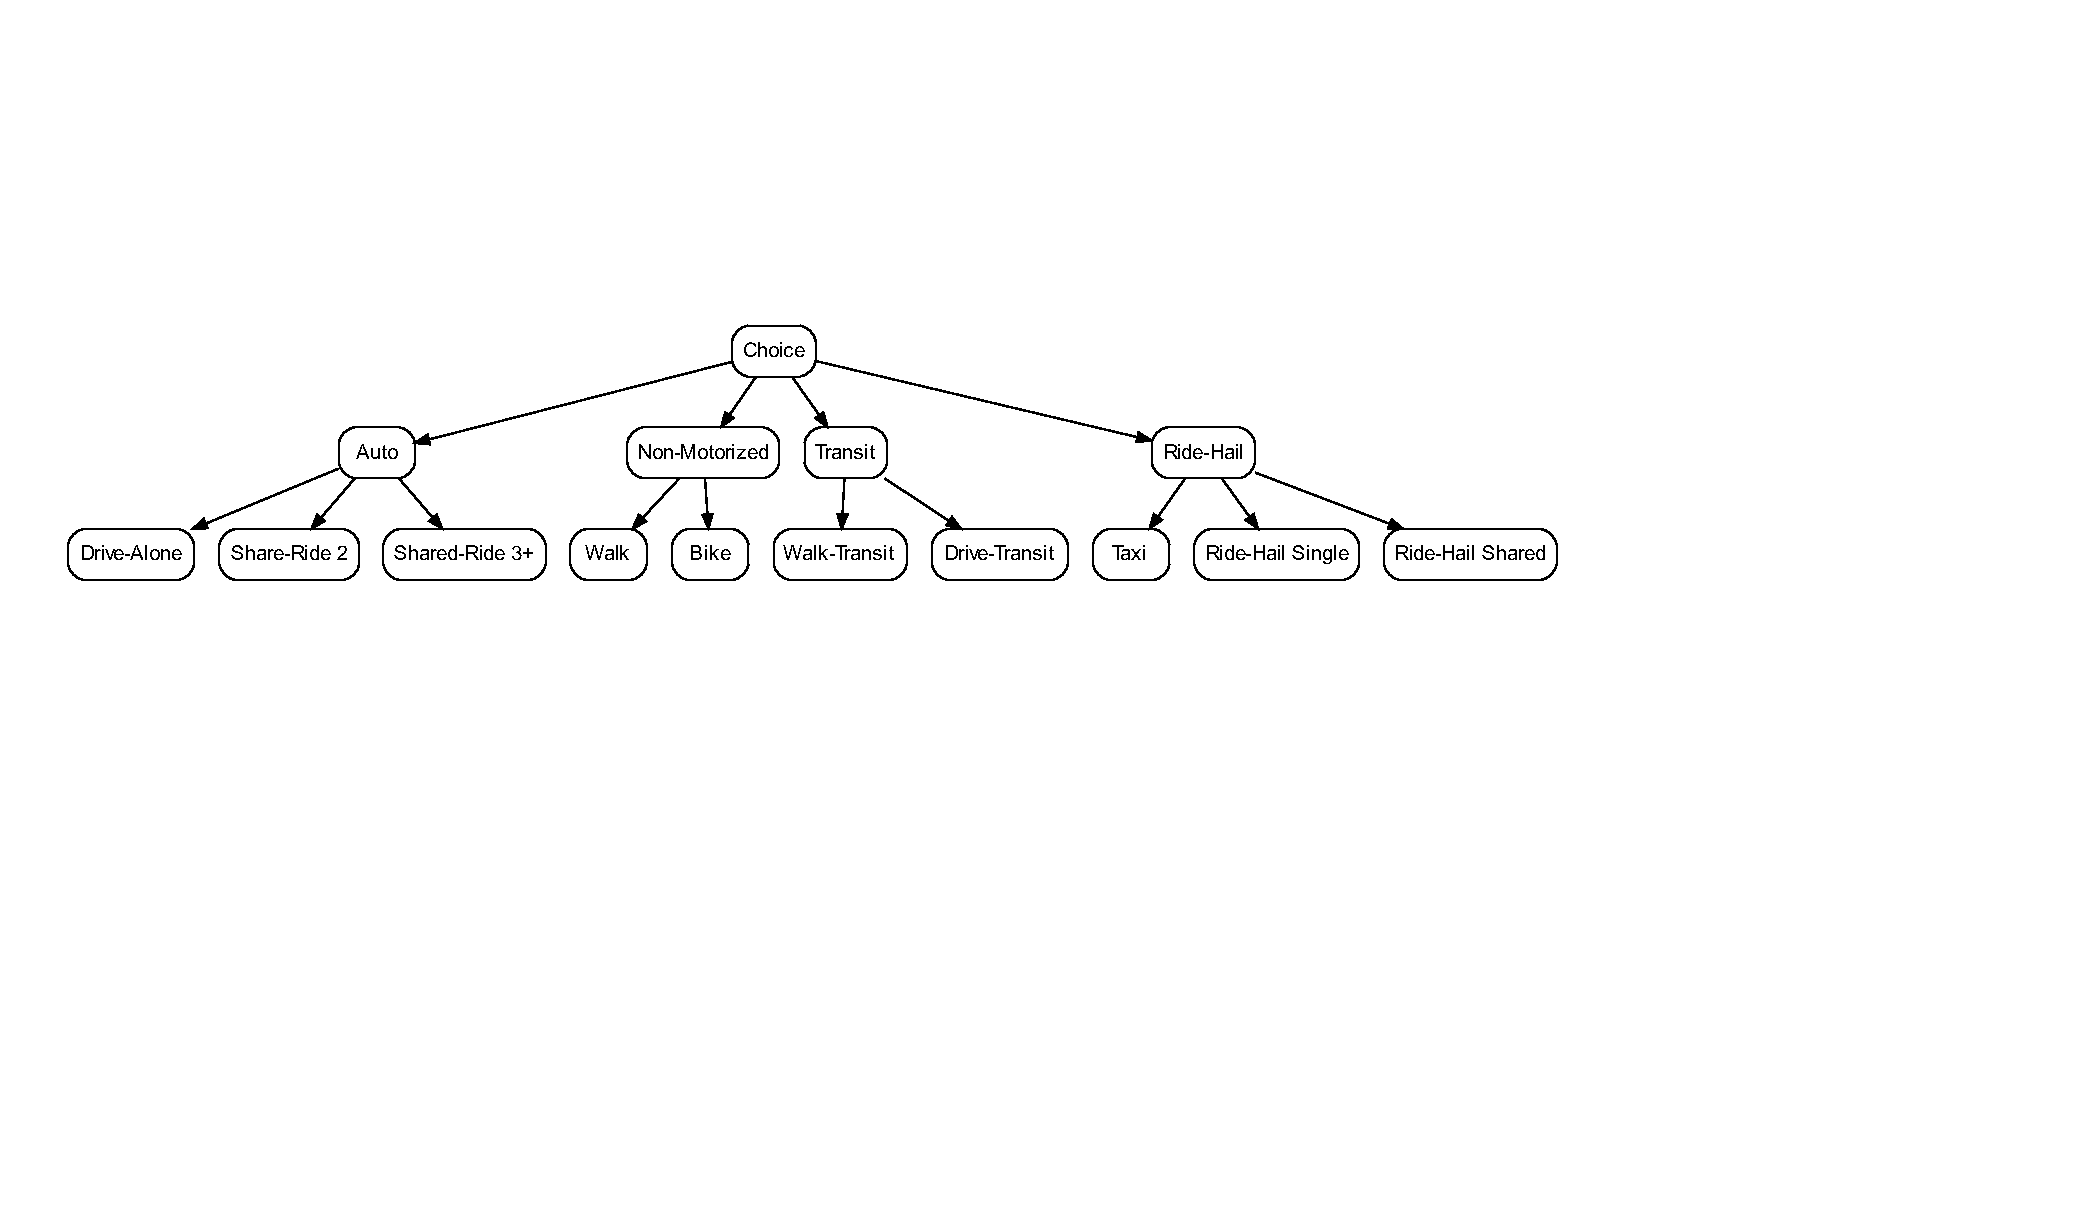
\includegraphics[width=.7\textwidth,trim = {5cm 6.5cm 12.5cm 4cm}]{thesis_files/figure-latex/fig-asim-nest-1} 

}

\caption{The nested logit model used in ActivitySim.}\label{fig:fig-asim-nest}
\end{figure}

Equation \eqref{eq:person} shows part of the ActivitySim's mode choice utility function that focuses on person variables. Equation \eqref{eq:path} shows the part of the mode choice utility function that focuses on path variables. (T stands for time, D stands for distance, and xfer stands for number of transfers). Equation \eqref{eq:location} shows the part of the mode choice utility function that focuses on location variables. (ZDI stands for zonal density index, ZTI stands for zonal topology index, and CBD stands for central business district). As shown in Equation \eqref{eq:all}, ActivitySim uses the combination of person, path, and location variables to calculate the mode choice alternative. The combination of these different variable types determines whether or not a person selected a ride-hailing mode. In addition, since activity-based models do not use variable wait time, the average wait time is selected before the model run.

\begin{equation}
  V_{Person} = ASC_{AutoOwnership} + \beta_{Cost}(Cost) + \beta_{Age}(Age) \label{eq:person}
\end{equation}

\begin{equation}
 V_{Path} = \beta_{TV}(T_{Vehicle}) + \beta_{TW}(T_{Wait}) + \beta_{TE}(T_{Egress}) + \beta_{TP}(TransitProx) + \newline \beta_{xfer}(xfer) + \beta_{DW}(D_{Walk}) + \beta_{DB}(D_{Bike}) + \beta_{DD}(D_{Drive}) \label{eq:path}
\end{equation}

\begin{equation}
  V_{Location} = \beta_{ZDI}(ZDI) + \beta_{ZTI}(ZTI) + \beta_{CBD}(CBD) \label{eq:location}
\end{equation}

\begin{equation}  
  V_{Mode} = Eq:2 + Eq:3 + Eq:4 \label{eq:all}
\end{equation}

\hypertarget{configuring-activitysim}{%
\subsection{Configuring ActivitySim}\label{configuring-activitysim}}

We configured ActivitySim to the case study region by first gathering and generating the input data. We needed the following three input files in order to run ActivitySim:

\begin{enumerate}
\def\labelenumi{\arabic{enumi}.}
\tightlist
\item
  A synthetic population of the agents within the study area.
\item
  A zonal socioeconomic data file describing the characteristics of each zone.
\item
  A set of skims that describe the cost and travel times of all modes between all zones.
\end{enumerate}

A synthetic population is a generated population with specific individual attributes that add up to the regional characteristics as a whole. We generated the synthetic population using a software called PopulationSim (PopulationSim, 2021). We used a ``seed'' table, which represented information of a subset of the population, and a set of ``targets'', which represented demographic data of smaller areas of the region, to run PopulationSim (Lant, 2021). The zonal socioeconomic data file stores zonal characteristics regarding household, worker, and other activity type information. We created this file using data from Wasatch Front Regional Council (WFRC) (WFRC, 2019), Utah Automated Geographic Reference Center (AGRC, 2021), and the synthetic population when necessary. The skims are large matrices showing travel times and costs between every set of zones within the area of study. Included in these skims were further details regarding differences in modes, distances, wait times, etc. (Lant, 2021). We used pre-generated skims from WFRC (2019), with some slight adjustments, in our run of the ActivitySim model.

After generating the necessary input files, we calibrated and validated the ActivitySim model to better represent decisions made in the Salt Lake region. The process of calibrating and validating the ActivitySim model to the Salt Lake region was conducted by Lant (2021). The purpose of the calibration and validation was to ensure that the outputs generated by ActivitySim matched target regional values. Specifically, trip productions, trip distributions, and mode choices were tested to match the given target values provided in the four-step model from WFRC (2019). The details behind the exact calibration and validation process are discussed by Lant (2021), and therefore will not be described in detail within this paper.

\hypertarget{meth-beam}{%
\section{BEAM as the Multi-agent Simulation}\label{meth-beam}}

BEAM stands for Behavior, Energy, Autonomy, and Mobility and is a multi-agent simulation being developed by Lawrence Berkeley National Laboratory and UC Berkeley Institute for Transportation Studies (BEAM, 2022). As an extension of MATSim, it simulates individual agents using both within day replanning and across-day replanning to maximize individual utility. Overall, BEAM shares many of the same advantages and disadvantages of most multi-agent simulations as described in Section \ref{lit-mas}.

\hypertarget{novel-beam}{%
\subsection{Ride-hailing in BEAM}\label{novel-beam}}

BEAM was chosen as the multi-agent simulation in this research because of its integration with transportation network companies (TNCs), or ride hail and pooled ride hail vehicles. Along with the TNC type mode options, BEAM supports many of the regular choices as well, such as car, walk, bike, walk-to-transit, and drive-to-transit. The default BEAM version uses a simple multinomial logit choice model to determine which mode any particular agent will use on any particular trip. The default version of BEAM also uses only a few variables to calculate the modal alternative, as seen in Equation \eqref{eq:beam} (BEAM, 2022).

\begin{equation}
  V_{Mode} = ASC_{Mode} + \beta_{Cost}(Cost) + \beta_{TV}(T_{Vehicle}) + \beta_{xfer}(xfer) \label{eq:beam}
\end{equation}

However, in order to better estimate the ride-hailing choices of individuals, the default BEAM mode choice model was improved upon. Specifically, the BEAM mode choice model was further developed to use a tour purpose attribute, the same utility equations as ActivitySim (See Equation \eqref{eq:all}), and additional modal alternatives consistent with those present in ActivitySim. A deeper explanation of these changes is provided in Appendix A (Section \ref{apexA}).

In addition to having a consistent mode choice structure with that of ActivitySim, BEAM implements ride-hailing vehicular behavior and assignment. BEAM uses a greedy asynchronous ride-hailing matching algorithm that also supports pooled trips (BEAM, 2022). The algorithm works by first, requiring agents to send a request for a ride hail vehicle, and then by second, matching the closest vehicle to that agent. For the algorithm to work, BEAM requires the modeler to input a ride hail vehicle fleet. This fleet is a simple file that describes the number of ride hail vehicles available in the region, their starting locations, their working hours, their seating capacity, and other specifications. BEAM assigns these vehicles to the roadway network, where they ``roam'' the streets awaiting requests. The ride hail algorithm permits a more realistic ride hail modeling structure. For example, agents make a request to take a ride hail vehicle, expect a variable wait time dependent on their geographic location, and may not even be able to take the vehicle if there is no availability. All these attributes are similar to how using ride-hailing is in real life, and represent the true advantages to modeling ride-hailing ridership and level of service with BEAM.

\hypertarget{configuring-beam}{%
\subsection{Configuring BEAM}\label{configuring-beam}}

BEAM was configured to the case study region by gathering the inputs, validating the utility parameter values, and calibrating the utility alternative specific constants (ASC) to match regional totals. BEAM input files were directly generated by the calibrated ActivitySim model. The utility parameter coefficients used in BEAM's mode choice model were copied directly from MTC's implementation of ActivitySim (MTC, 2012). MTC's implementation of ActivitySim was designed for the San Francisco, California region. Logically, travel behaviors such as travel time, travel distance, and number of transfers should affect people in different regions in similar ways. However, as a way to validate the use of ActivitySim's path utility coefficients in the Salt Lake region, we compared these values to values from the Utah Statewide model (UDOT, 2021), the WFRC travel demand model (WFRC, 2019), and NCHRP Report 716 (Cambridge Systematics et al., 2012). The Utah Statewide model provided a rough idea of the influence of path variables in Utah as a whole. The WFRC model model provided a direct comparison of travel behavior for the same region of study used in this research. NCHRP Report 716 provided a rough idea of what parameter values should look like from a generalized modeling point of view. Overall, comparing these three sets of path parameter values with the MTC ActivitySim parameter values used in BEAM helped ensure that the the mode choice utility parameters were valid.

Figure \ref{fig:coef} shows the comparison of the path utility parameter values between all four models for home-based work, home-based school, and home-based other trips. To view all parameters on the same scale, each value is divided by the in vehicle travel time (IVTT) coefficient. For the egress time, IVTT, the number of transfers, transfer time, and the wait times, MTC's ActivitySim seems to use a very similar coefficient value as the other three models. The largest discrepancy exists with short and long walking distances. ActivitySim seems to use a value almost ten fold that of the other models. This occurs because the WFRC and Utah Statewide models cap walking distance whereas ActivitySim instead gives a high penalty for long walking distances. With this clarification, it is clear to see that ActivitySim's path coefficient values do not require calibration and were left as is because the parameters fall within a close range of the other models.

\begin{figure}

{\centering 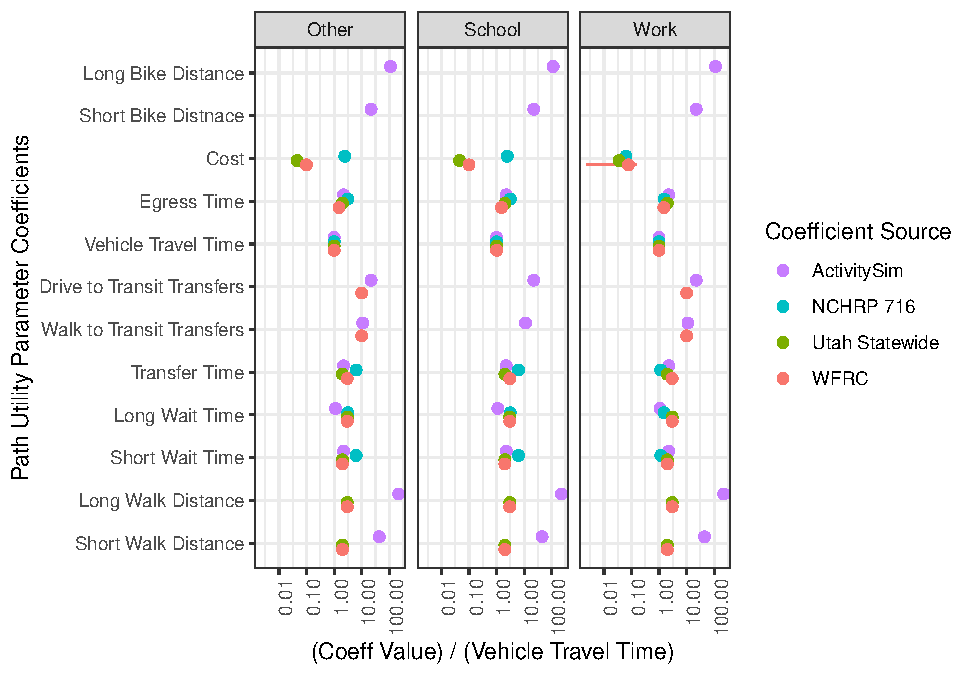
\includegraphics{thesis_files/figure-latex/coef-1} 

}

\caption{Mode choice path coefficients model comparison by tour purpose.}\label{fig:coef}
\end{figure}

Lastly, after completing the utility parameter validation we calibrated the mode choice utility function's ASC values. We completed BEAM calibration by iteratively updating the ASC values using Equation \eqref{eq:eqcalib}. We compared the number of trips totaled by tour purpose, auto ownership, and modal alternative between the BEAM results and the ActivitySim results to adjust each ASC value. After completing 15 iterations of compouding Equation \eqref{eq:eqcalib} on the ASC values, the BEAM trip values were within a reasonable range to the ActivitySim target shares. Figure \ref{fig:fig-beam-calib} shows the progress of the calibration targets with the final shares after each iteration.

\begin{equation}
  NewASC = OldASC + ln(\frac{Trips_{ASIM}}{Trips_{BEAM}}) \label{eq:eqcalib}
\end{equation}

\begin{landscape}

\begin{figure}[H]
\centering
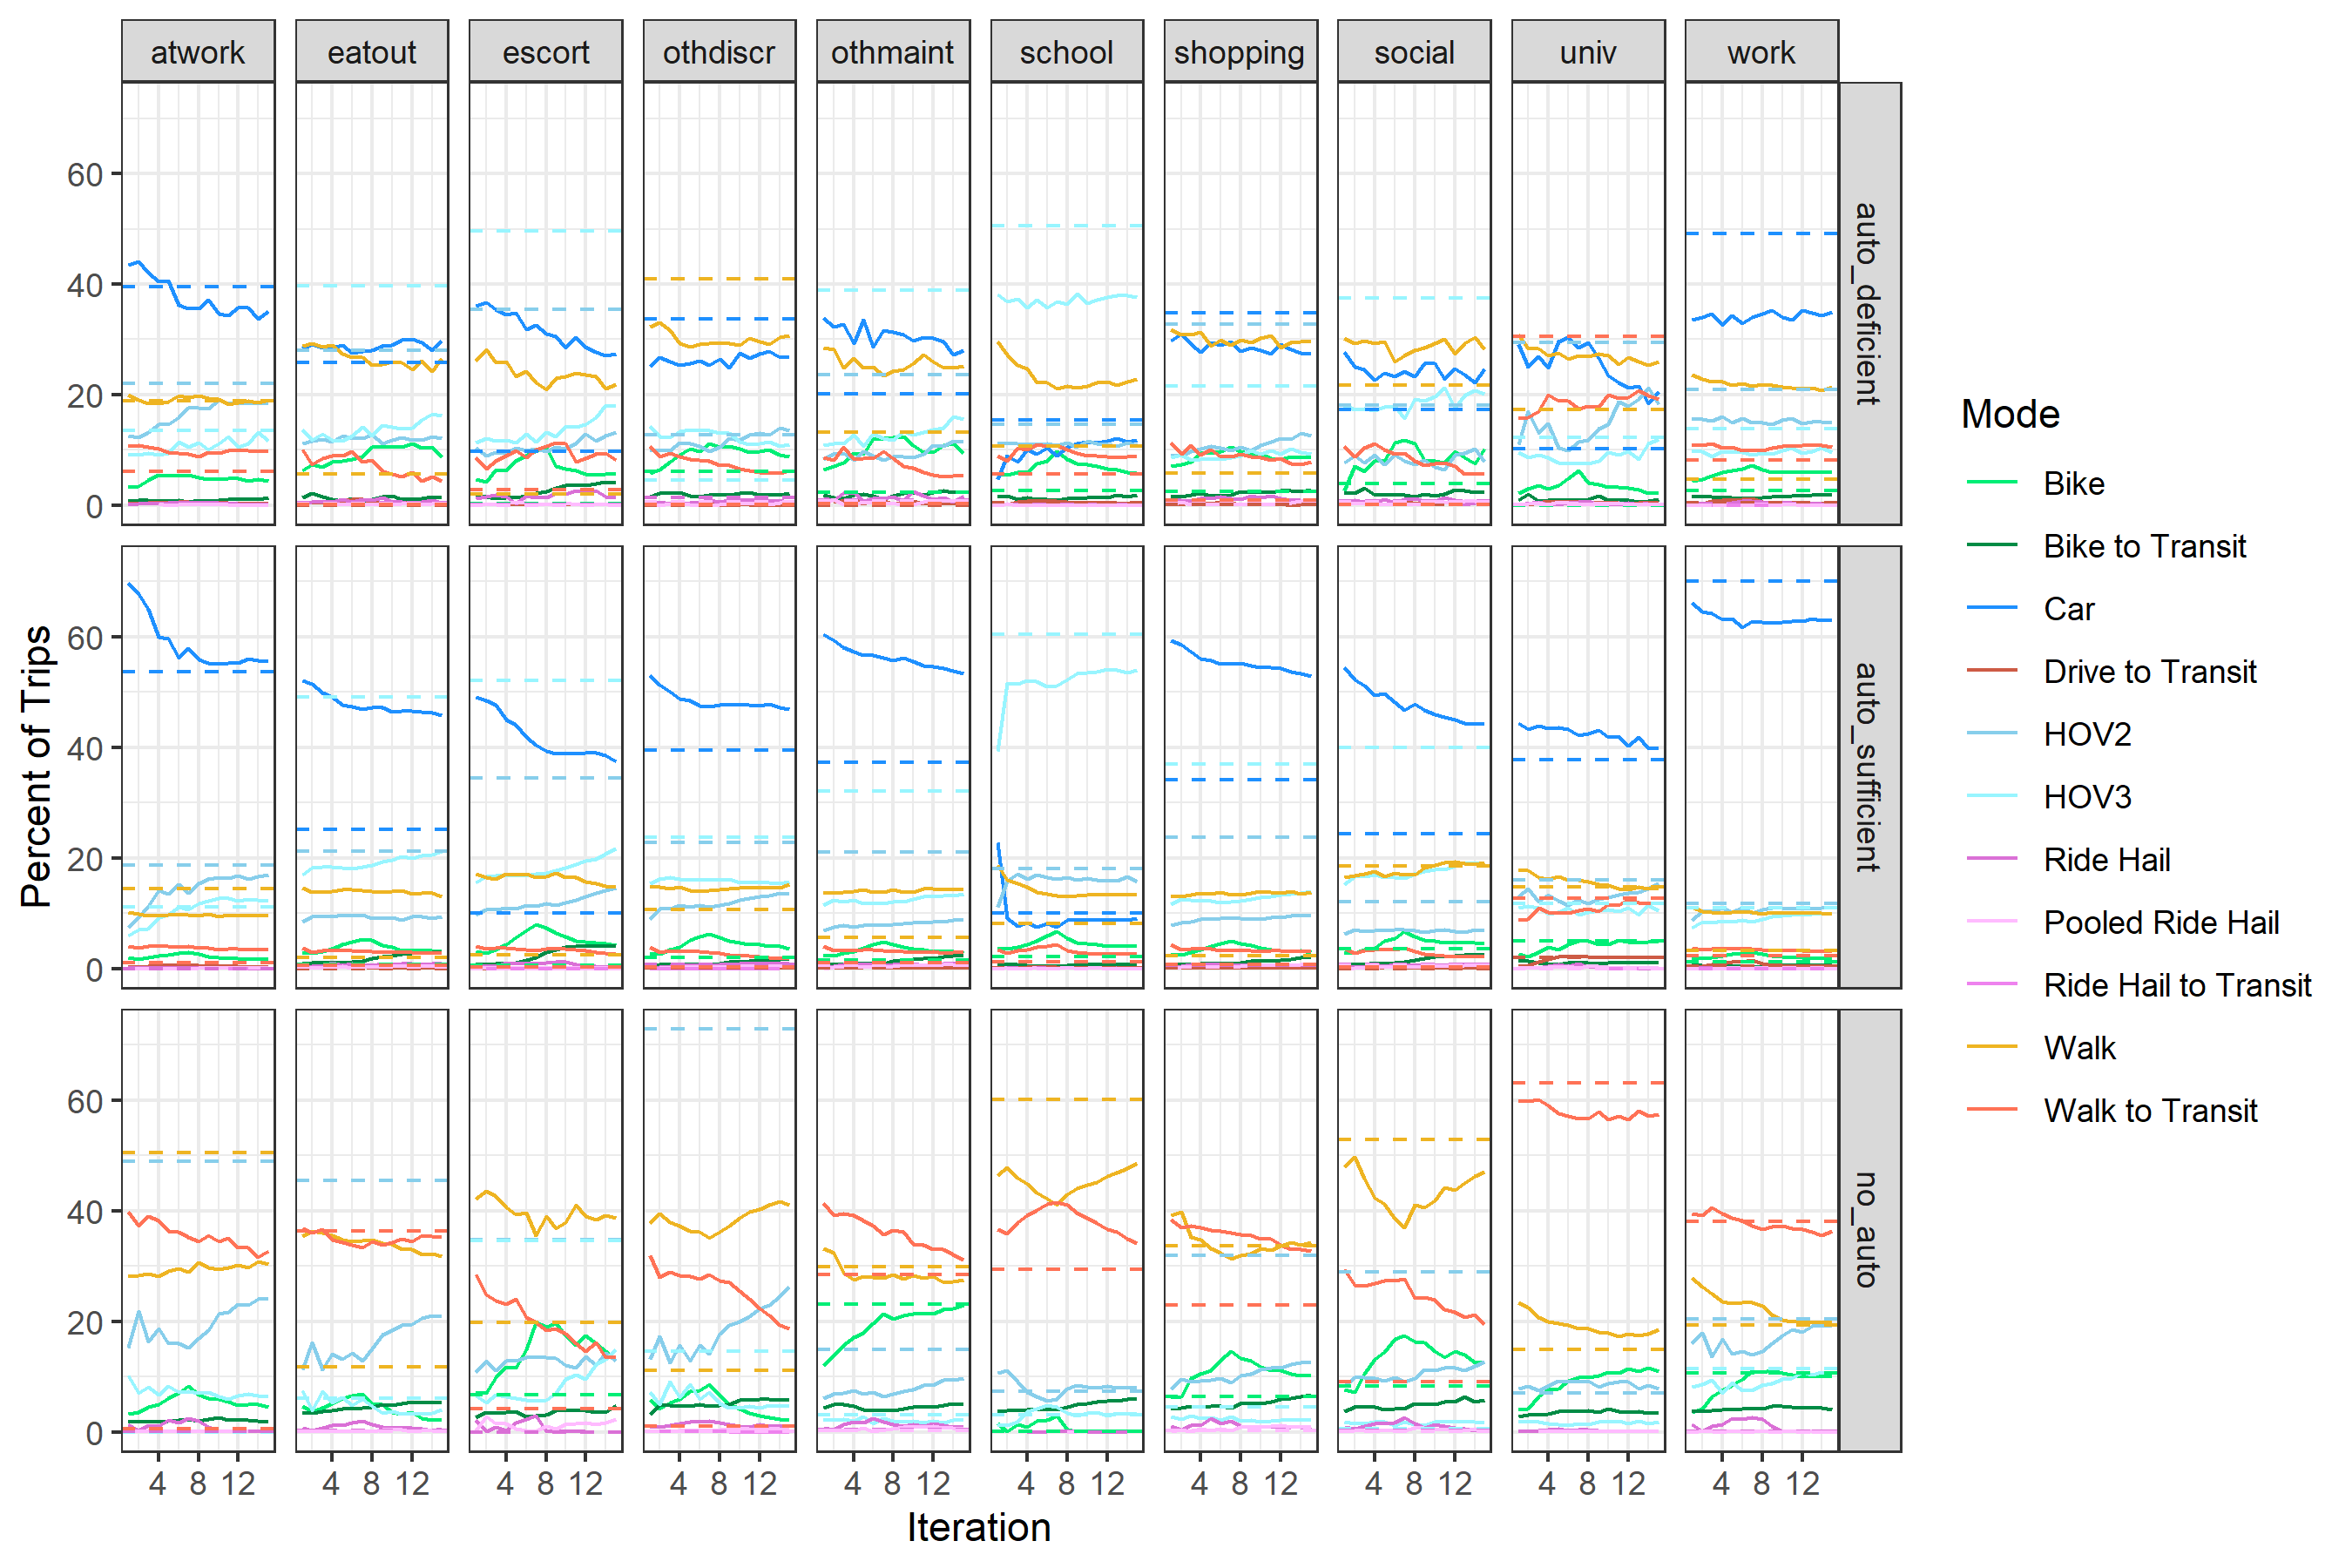
\includegraphics{pics/BeamCalib.png}
\caption{BEAM mode choice ASC calibration.}
\label{fig-beam-calib}
\end{figure}

\end{landscape}

\hypertarget{meth-scenarios}{%
\section{Case Study Scenarios}\label{meth-scenarios}}

After completing the BEAM validation and BEAM calibration for the case study region, we ran a series of different BEAM experiments. We ran each experiment for a total of 12 iterations using a 15\% population size. More specifically, we ran 9 different experiments, each with a unique ActivitySim-to-BEAM mode choice combination. Table \ref{tab:tbexperiments} provides a short name description of the 9 different scenarios.

\begin{table}
\caption{ActivitySim-to-BEAM Mode Choice Combination Scenario Names}
\renewcommand{\arraystretch}{2}
\[
  \begin{array}{cc|ccc}
    &\multicolumn{1}{c}{} & \multicolumn{2}{c}{\text{ActivitySim}} \\
    && \text{Plans without Ride Hail} & \text{Plans with RideHail}\\
    \hline
    & \text{None} & \text{} & \text{AsimRideHail} \\
    \smash{\rotatebox[origin=c]{90}{\text{BEAM}}} & \text{RideHail} & \makecell{\text{BeamRideHail:Path} \\ \text{BeamRideHail:PPL}} & \makecell{\text{AsimBeamRideHail:Path} \\ \text{AsimBeamRideHail:PPL}} \\
    & \text{All} & \makecell{\text{BeamAll:Path} \\ \text{BeamAll:PPL}} & \makecell{\text{AsimBeamAll:Path} \\ \text{AsimBeamAll:PPL}}
  \end{array}
\]
\label{tab:tbexperiments}
\end{table}

To better describe the meaning of each scenario in Table \ref{tab:tbexperiments}, we explain the three mode choice descriptors that were altered in each scenario. The first descriptor refers to how ActivitySim's modes were configured, which in Table \ref{tab:tbexperiments} is labeled under \emph{ActivitySim} as \emph{Plans without RideHail} and \emph{Plans with RideHail}. In the naming convention, any name starting with \emph{Asim} refers to any scenario where ride-hailing was included in the input plans from ActivitySim, and any name without \emph{Asim} refers to any a scenario where ride-haling was excluded from the inputs plans from ActivitySim. In other words, the ActivitySim ride-hailing nesting option as shown in Figure \ref{fig:fig-asim-nest} only existed in one version of ActivitySim. Since the daily activity plans generated by ActivitySim were converted to BEAM inputs, this descriptor explains the initial mode choice selections for all trips entered into BEAM.

The second descriptor present in Table \ref{tab:tbexperiments} is labeled under \emph{BEAM} as \emph{None}, \emph{RideHail}, and \emph{All}. These three variables explain which mode choice structure was used in BEAM. These variables also explain which modal alternatives were available for choice within BEAM. The \emph{None} category represents a version of BEAM where all modal innovation was turned off. This means that no mode choice was available, and the modes from the initial input plans remained constant across each iteration. The \emph{RideHail} category represented a version of BEAM where modal innovation was partially turned off. All trips that originally took car or carpool modes had modal innovation turned off; their modes were locked. All trips that originally took walk-transit or drive-transit modes, however, were given the option to switch to a ride-haliing mode. Also, all walk modes were given the option to switch to a ride hail vehicle. \emph{RideHail} represents the version of BEAM where ride hail and ride hail transit modes were only given to none-car dependent agents. Finally, the \emph{All} category represents a version of BEAM where modal innovation was turned on, and all modal alternatives were available for choice. This means that within-day replanning as well as across-day replanning was turned on, and agents could change their trip modes to maximize their utility.

Finally, the third descriptor present in Table \ref{tab:tbexperiments} is labeled as either \emph{Path} or \emph{PPL} and explains which utility variables were used to calculate modal utility. The options include \emph{Path}, \emph{PPL}, and empty. The empty option means no utility parameters were used in determining mode choice, because modal innovation was turned off completely. The \emph{Path} option represented the version of BEAM that only used path type utility parameters to calculate mode choice utility; location and person type variables were not used (See Equation \eqref{eq:path}). The \emph{PPL} option represented the version of BEAM that used all utility parameter types (Path, Person, and Location) to calculate the mode choice utility (See Equation \eqref{eq:all}).

Overall, we ran 9 different scenarios each with a slightly different ActivitySim-to-BEAM mode choice combination. Each scenario is built from which modes were included in the input plans, which modal alternatives were available for choice, and which utility parameter types were used to calculate the mode choice utility. By altering these three different mode choice characteristics, we hope to better understand the affect a linked activity-based model and multi-agent simulation have on ride-hailing riderhsip and level of service.

\hypertarget{results}{%
\chapter{Results}\label{results}}

We estimated ride-hailing ridership and level of service for each of the 9 previously mentioned ActivitySim-to-BEAM mode choice combinations. Specifically, we estimated ride-hailing ridership, wait time, and utilization. Alongside each other, these results shed light on the performance of estimating ride-haling ridership and level of service with an activity-based model and multi-agent simulation. We can see how differing mode choice structures affect the use and performance of ride-hailing modes.

\hypertarget{res-ridership}{%
\section{Ridership}\label{res-ridership}}

Table \ref{tab:ridership} shows the number of trips for the ride hail, pooled ride hail, and ride hail transit type modes for all 9 mode choice combinations. Table \ref{tab:ridership} also includes the number of trips within the plans with ride hail created by ActivitySim, before the mode choices were changed by the BEAM.

\begin{landscape}\begin{table}

\caption{\label{tab:ridership}Ride Hail Ridership by Number of Total Trips by Mode Choice Combination.}
\centering
\begin{tabular}[t]{lrrrr}
\toprule
Scenario Name & Ride Hail & Pooled Ride Hail & Ride Hail to Transit & Total\\
\midrule
\cellcolor[HTML]{D9D9D9}{\em{ActivitySim}} & \cellcolor[HTML]{D9D9D9}{\em{2412}} & \cellcolor[HTML]{D9D9D9}{\em{1837}} & \cellcolor[HTML]{D9D9D9}{\em{0}} & \cellcolor[HTML]{D9D9D9}{\em{4249}}\\
\cellcolor[HTML]{FAEBD7}{AsimRideHail} & \cellcolor[HTML]{FAEBD7}{269} & \cellcolor[HTML]{FAEBD7}{31} & \cellcolor[HTML]{FAEBD7}{0} & \cellcolor[HTML]{FAEBD7}{300}\\
\cellcolor[HTML]{FFB6C1}{BeamRideHail:Path} & \cellcolor[HTML]{FFB6C1}{45001} & \cellcolor[HTML]{FFB6C1}{25014} & \cellcolor[HTML]{FFB6C1}{2943} & \cellcolor[HTML]{FFB6C1}{72958}\\
\cellcolor[HTML]{FFB6C1}{BeamRideHail:PPL} & \cellcolor[HTML]{FFB6C1}{18907} & \cellcolor[HTML]{FFB6C1}{38935} & \cellcolor[HTML]{FFB6C1}{4621} & \cellcolor[HTML]{FFB6C1}{62463}\\
\cellcolor[HTML]{FFB6C1}{AsimBeamRideHail:Path} & \cellcolor[HTML]{FFB6C1}{21519} & \cellcolor[HTML]{FFB6C1}{40873} & \cellcolor[HTML]{FFB6C1}{5437} & \cellcolor[HTML]{FFB6C1}{67829}\\
\addlinespace
\cellcolor[HTML]{FFB6C1}{AsimBeamRideHail:PPL} & \cellcolor[HTML]{FFB6C1}{47422} & \cellcolor[HTML]{FFB6C1}{27327} & \cellcolor[HTML]{FFB6C1}{3848} & \cellcolor[HTML]{FFB6C1}{78597}\\
\cellcolor[HTML]{ADD8E6}{BeamAll:Path} & \cellcolor[HTML]{ADD8E6}{4671} & \cellcolor[HTML]{ADD8E6}{1596} & \cellcolor[HTML]{ADD8E6}{38} & \cellcolor[HTML]{ADD8E6}{6305}\\
\cellcolor[HTML]{ADD8E6}{BeamAll:PPL} & \cellcolor[HTML]{ADD8E6}{3146} & \cellcolor[HTML]{ADD8E6}{6366} & \cellcolor[HTML]{ADD8E6}{121} & \cellcolor[HTML]{ADD8E6}{9633}\\
\cellcolor[HTML]{ADD8E6}{AsimBeamAll:Path} & \cellcolor[HTML]{ADD8E6}{3470} & \cellcolor[HTML]{ADD8E6}{4596} & \cellcolor[HTML]{ADD8E6}{90} & \cellcolor[HTML]{ADD8E6}{8156}\\
\cellcolor[HTML]{ADD8E6}{AsimBeamAll:PPL} & \cellcolor[HTML]{ADD8E6}{3153} & \cellcolor[HTML]{ADD8E6}{6031} & \cellcolor[HTML]{ADD8E6}{156} & \cellcolor[HTML]{ADD8E6}{9340}\\
\bottomrule
\end{tabular}
\end{table}
\end{landscape}

By comparing scenarios amongst each other, we can understand how slight differences in the mode choice model can significantly affect ridership totals. We first compare the AsimRideHail scenario with the ActivitySim scenario. Comparing these two scenarios we see how BEAM severely undercuts the number of ride-hailing trips estimated in the input plans generated by ActivitySim. ActivitySim estimated a total of 4249 ride-hailing trips whereas the AsimRideHail scenario only estimated 300. Even with no mode choice model in BEAM, by simply running ActivitySim's ride-hailing estimates in the BEAM environment, BEAM was unable to create ride-hailing paths in most cases.

On the other hand, by comparing the AsimRideHail scenario with the \emph{RideHail} type scenarios we see that the ridership totals are greather than in the AsimRideHail scenario. The BEAM mode choice structure which allows only ride hail modal innovation will predict significantly higher ridership totals than both ActivitySim and AsimRideHail. Then, by comparing the AsimRideHail scenario with the BeamAll scenarios we see the effectiveness of BEAM at estimating ride hail modes without ride hail being selected in the initial plans. Both BeamAll scenarios display a large increase in total ride hail ridership when compared with the AsimRideHail scenario. Also, by comparing the \emph{All} type scenarios, we notice that BEAM will estimate higher ridership totals than AsimRideHail and ActivitySim, independent of whether or not the input plans include ride hailing modes.

Interestingly, by comparing the AsimRideHail scenario with the AsimBeamAll:PPL scenario we learn about the inter-workings of the BEAM mode choice that is most consistent with ActivitySim. The BeamAll:PPL and AsimBeamAll:PPL scenarios reference a BEAM mode choice structure which uses the same modal options and utility parameters as ActivitySim. By comparing AsimBeamAll:PPL with the AsimRideHail scenario, we see how ride hail statistics \emph{differ} when modeled with an activity-based model than with a multiagent simulation. Looking at the differences between the ActivitySim and AsimBeamAll:PPL scenarios in Table \ref{tab:ridership}, we see an increase of 5091 trips by simply turning on modal innovation in BEAM. We conclude that BEAM is more prone to estimating higher ridership totals for ride hailing modes than ActivitySim when modal innovation is turned on.

Next, by analyzing the collective groups within the table, we can extract deeper results. First, we examine the effect of ride-hailing existing in the input plans. As shown in Table \ref{tab:ridership}, minimal differences in ridership is produced between scenarios with the \emph{Asim} prefix vs.~without. For example, with the BeamRideHail:Path and AsimBeamRideHail:Path, we see that when ride hail doesn't exist in the input plans, the total ride-hailing trips is 72,958 whereas when ride hail type modes are included, the total ride-hailing modes is 67,829 trips. Both scenarios project an enormous share of ride-hailing trips. Similarly, the gap between the ride-hailing trips of the BeamRideHail:PPL and AsimBeamRideHail:PPL scenario is relatively close, at 62,463 and 78,597 trips respectively. Then, when examining BeamAll:PPL and AsimBeamAll:PPL, the output ridership percentages are almost identical; similarly, the ride-hailing trip totals of the BeamAll:Path and AsimBeamAll:Path scenarios are close. Overall, by collectively comparing all the scenarios with ride-hailing input plans against those without, we see similar ridership results among similar mode choice structures.

Although input plans do not seem to have a significant effect on ridership, the BEAM mode choice strucutres do. The \emph{None} type scenario (AsimRideHail) produces little to no agents choosing ride hail. On the other hand, the \emph{RideHail} type scenarios produce the largest number of ride hail modes amoung BEAM mode choice structures. The \emph{All} type scenarios produce a significantly larger number of ride hail modes than the \emph{None} type, but a singificantly lower numer of ride hail modes than the \emph{RideHail} type. In addition, the \emph{All} type scenarios seem to predict similar ridership values with ActivitySim. For example, the number of ride hail only type trips is 2,259 more in the BeamAll:Path scenario than in the ActivitySim scenario. Ridership is affected significantly by which mode choice structure is used by BEAM; this conclusion is clear.

Finally, we analyze the effect the BEAM utility variables have on ride hail ridership totals. We first compare the BeamRideHail:Path and BeamRideHail:PPL scenarios. In this case, ride hail only ridership decreases (45,001 and 18,907) when using path, person, and location variables, but increases with pooled ride hail (25,014 and 38,935) and ride hail transit (2,943 and 4,621) when using path, person, and location variables. This same pattern occurs when analyzing the difference between the BeamAll:Path and BeamAll:PPL, and AsimBeamAll:Path and AsimBeamAll:PPL scenarios. For some oddity, AsimBeamRideHail:Path and AsimBeamRideHail:PPL follow an opposite pattern where ride hail increases (21,519 and 47,422) and ride hail pooled decreases (40,873 and 27,327) and ride hail transit decreases (5,437 and 3,848) when using path, person, and location variables. We acknowledge that not all scenarios follow the same pattern, but hypothesize that in general, using only path variables to estimate ride hail ridership will result in less total ride hail ridership than if using all path, person, and location type variables.

\hypertarget{res-waits}{%
\section{Wait Times}\label{res-waits}}

Figure \ref{fig:waits} shows the results of wait times for ride-hailing vehicles for the scenarios that were run. By analyzing the wait times with violin plots, we see a detailed distribution of the ride-hailing wait times for each scenario.

\begin{figure}

{\centering 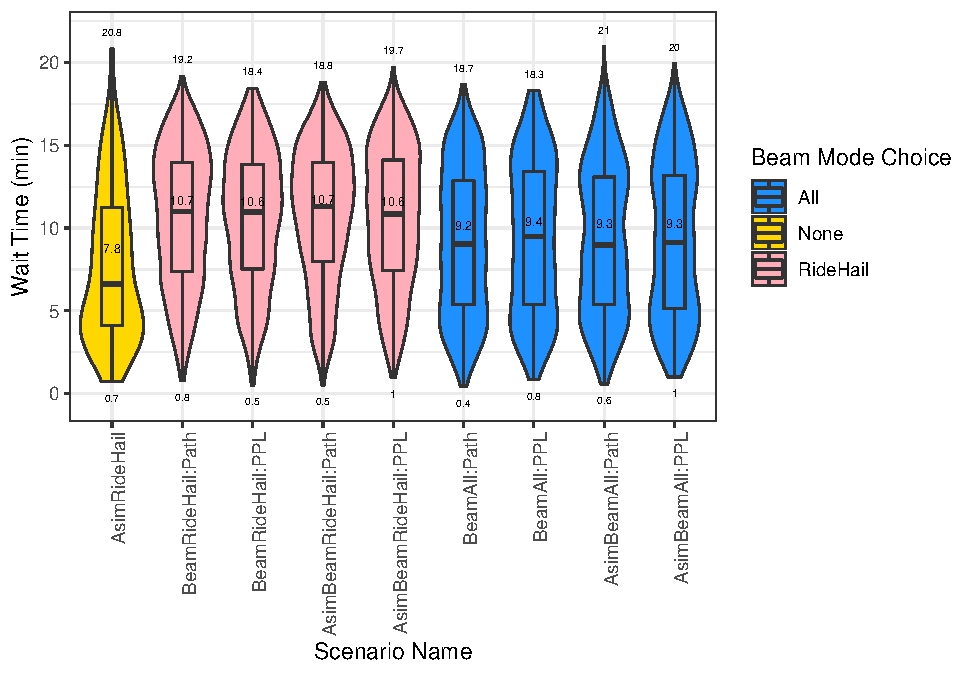
\includegraphics{thesis_files/figure-latex/waits-1} 

}

\caption{Distribution of ride hail wait times by mode choice combination scenario.}\label{fig:waits}
\end{figure}

As was done in Section \ref{res-ind}, we can compare scenarios between one another For example, when looking at the AsimRideHail and AsimBeamAll:PPL scenairio, we see that wait times increase when using the BEAM mode choice model (minimum wait time increases from 0.7 to 1 minute, and mean wait time increases from 7.8 to 9.3 minutes). A noticeable increase in wait time is achieved by simply turning on modal innovation in BEAM. Since higher wait time suggest higher ridership, we conclude that BEAM is prone to estimating more ride hail usage than ActivitySim when modal innovation is turned on. Then, by comparing AsimRideHail and BeamAll:PPL we see the lack of impact that ride hail in the initial plans has on effective ride hail usage. The wait time mean may have increased from 7.8 to 8.4 minutes, but the maximum wait time decreased from 20.8 to 18.3 minutes. Although no ride-hailing existed in the input plans, BEAM was effectively able to calculate the usage of more ride hail vehicles with less maximum wait times.

As with ridership, analyzing wait times on a collective scale sheds additional light how mode choice affects ride-hailing service capabilities. For example, collectively comparing the scenarios with the \emph{Asim} prefix against the scenarios without, we see a slight difference in maximum wait times. Scenarios AsimBeamRideHail:PPL, AsimBeamAll:Path, and AsimBeamAll:PPL have almost identical mean wait times when compared to their counterparts in BeamRideHail:PPL, BeamAll:Path, BeamAll:PPL. We suppose that the existence of ride hail in the initial plans will not affect \emph{most} ride hail wait times.

Alternately, comparing different BEAM mode options does significantly affect ride hail wait times. The \emph{None} type scenario (AsimRideHail) has the largest spread of wait times, the lowest mean wait time, and is ``bottom heavy'' -- referring to the fact that a major cluster of users wait less than 7.5 minutes. The \emph{All} type scenarios have higher mean wait times (\textasciitilde9.3 minutes) than the \emph{None} type and lower mean wait times than the \emph{RideHail} type. Neither top nor bottom heavy, the \emph{All} type scenarios seem to have a more even spread in wait times, ranging from 0.4 to 21 minutes. BEAM seems to paint ride hail alternatives as more desirable than ActivitySim, as more users are willing to wait longer (12 to 18 minutes in the \emph{All} scenarios). This is especially true with the \emph{RideHail} type scenarios, as a large cluster of users are willing to wait 7.5 to 20 minutes. The \emph{RideHail} type scenarios have the largest mean wait times (\textasciitilde10.65 minutes). Overall, wait time is significantly affected by which mode choice structure is used by BEAM, just like as was concluded with ridership.

The last group to compare collectively is between the Path and PPL models. By comparing BeamRideHail:Path and BeamRideHail:PPL, BeamAll:Path and BeamAll:PPL, and AsimBeamAll:Path and AsimBeamAll:PPL, we see that the Path models estimate a slightly higher maximum wait time. In addition, BeamRideHail:Path and AsimBeamRideHail:Path seem to have a larger cluster above a 10 minute wait time than BeamRideHail:PPL and AsimBeamRideHail:PPL. Besides these two observations though, the differences between utility parameters is minimal. Although ridership was affected by which utility parameters were used, wait time is only slightly affected.

\hypertarget{summary}{%
\subsection{Summary}\label{summary}}

Overall, by analyzing the ridership amd wait times among different mode choice structures we learn that ride-hailing ridership and level of service is significantly affected by which mode choice structure is used in BEAM. We also propose that initial plans, and whether or not they include ride hail, do not significantly affect the level at which BEAM estimates ridership, however it may affect service capabilities like wait time. Lastly, we hypothesize that using all path, person, and location type variables will increase total ridership. We also suggest that the lack of person attributes in the utility equation may cause pooled and transit ride hail options to look less appealing. Section \ref{deep-look} takes a deeper look at why some patterns in the ridership and wait times results exist.

\hypertarget{deep-look}{%
\section{A Deeper Look at Ridership and Wait Times}\label{deep-look}}

The results from Table \ref{tab:tbexperiments} and the results from Figure \ref{fig:waits} can be explained further by understanding the original setup of the experiments. The clearest distinction in ridership and wait times exist between BEAM mode choice structures. The \emph{None}, \emph{RideHail}, and \emph{All} structure types each produce results at different magnitudes. These vastly different results are directly related to how each model structure was constructed.

\hypertarget{type1}{%
\subsection{None Mode Choice Model}\label{type1}}

The \emph{None} mode choice model produces the lowest ridership and quickest wait time values. With modal innovation turned off, agents were unable to choose new modes, and averted to walk modes if the current trip mode was deemed ``impossible''. This is verified by looking at Table \ref{tab:noneloss}. Iteration 0 (start) shows the number of ride-hailing modes input to BEAM. By the end of iteration 0, however, more than half the initial ride-hailing selections estimated by ActivitySim were lost. Then, by the end of the final iteration, only 300 ride-hailing trips remained. At the same time, total walk modes increases across each iteration. BEAM was unable to match agents with most of ActivitySim's ride-hailing predictions.

\begin{table}

\caption{\label{tab:noneloss}Loss of Ride-hailing trips in the None Mode Choice Model.}
\centering
\resizebox{\linewidth}{!}{
\begin{tabular}[t]{lllll}
\toprule
Iteration & Ride Hail & Pooled Ride Hail & Ride Hail Transit & Total\\
\midrule
0 (start) & 2412 & 1837 & 0 & 4249\\
0 (end) & 978 & 615 & 0 & 1593\\
12 (end) & 269 & 21 & 0 & 300\\
\bottomrule
\end{tabular}}
\end{table}

\hypertarget{type3}{%
\subsection{All Mode Choice Model}\label{type3}}

The \emph{All} BEAM mode choice model uses the same mode choice utility function as ActivitySim and has all modal alternatives available. This adjusted model structure helps us understand why we obtained much higher ridership than with the \emph{None} Model. Figure \ref{fig:piechart} shows from which modes agents who switched to ride-hailing came from. Interestingly enough, the majority of agents who select ride hail switched from car type modes (Car, HOV2, HOV3).

\begin{figure}

{\centering 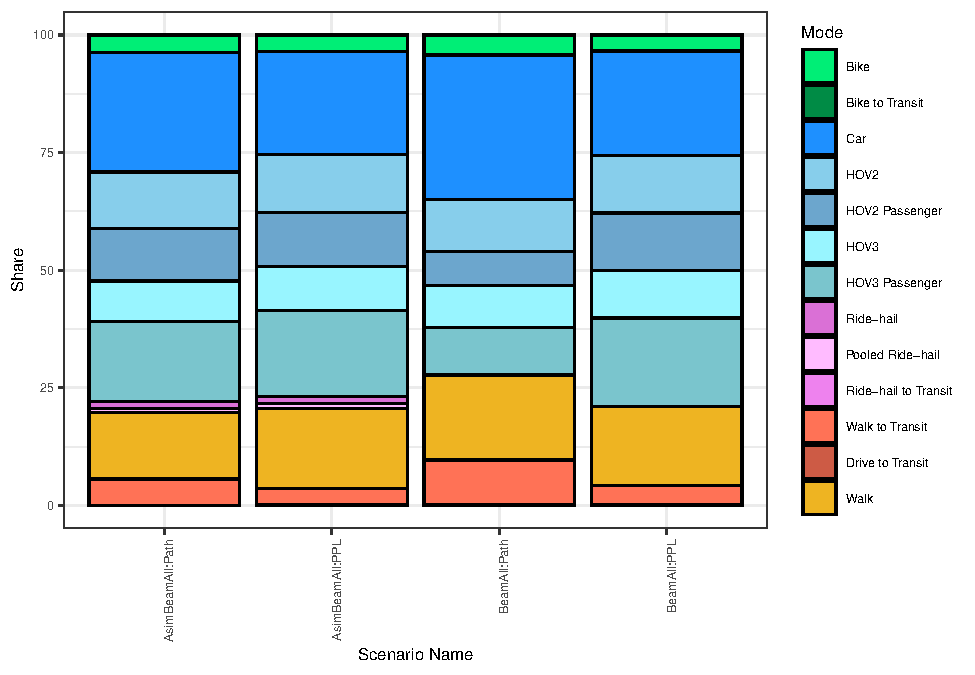
\includegraphics{thesis_files/figure-latex/piechart-1} 

}

\caption{Original mode choices of agents who switch to a ride hail type mode.}\label{fig:piechart}
\end{figure}

We offer three factors as to why so many car users switch to ride-hailing modes. The first is the array of utility parameters boosted the ride-hailing utility, making ride-hailing options attractive alternatives. Figure \ref{fig:sankey} provides sufficient evidence for this claim. Figure \ref{fig:sankey} shows a sankey diagram of all modal decisions at the start of each iteration for the AsimBeamAll:PPL scenario. The mode ``No Mode'' describes those modes that were cleared and reset at the beginning of each iteration. Notice how many of the Car, HOV2, HOV2 Passenger, HOV3, and HOV3 Passenger modes shift into the ``No Mode'' category each iteration. Also notice in the subsequent iteration how many of those ``No Mode'' choices shift to ride-hailing modes. A shift from the ``No Mode'' choice to ride hail represents those agents choosing their mode based on the utility value.

\begin{landscape}

\begin{figure}[H]
\centering
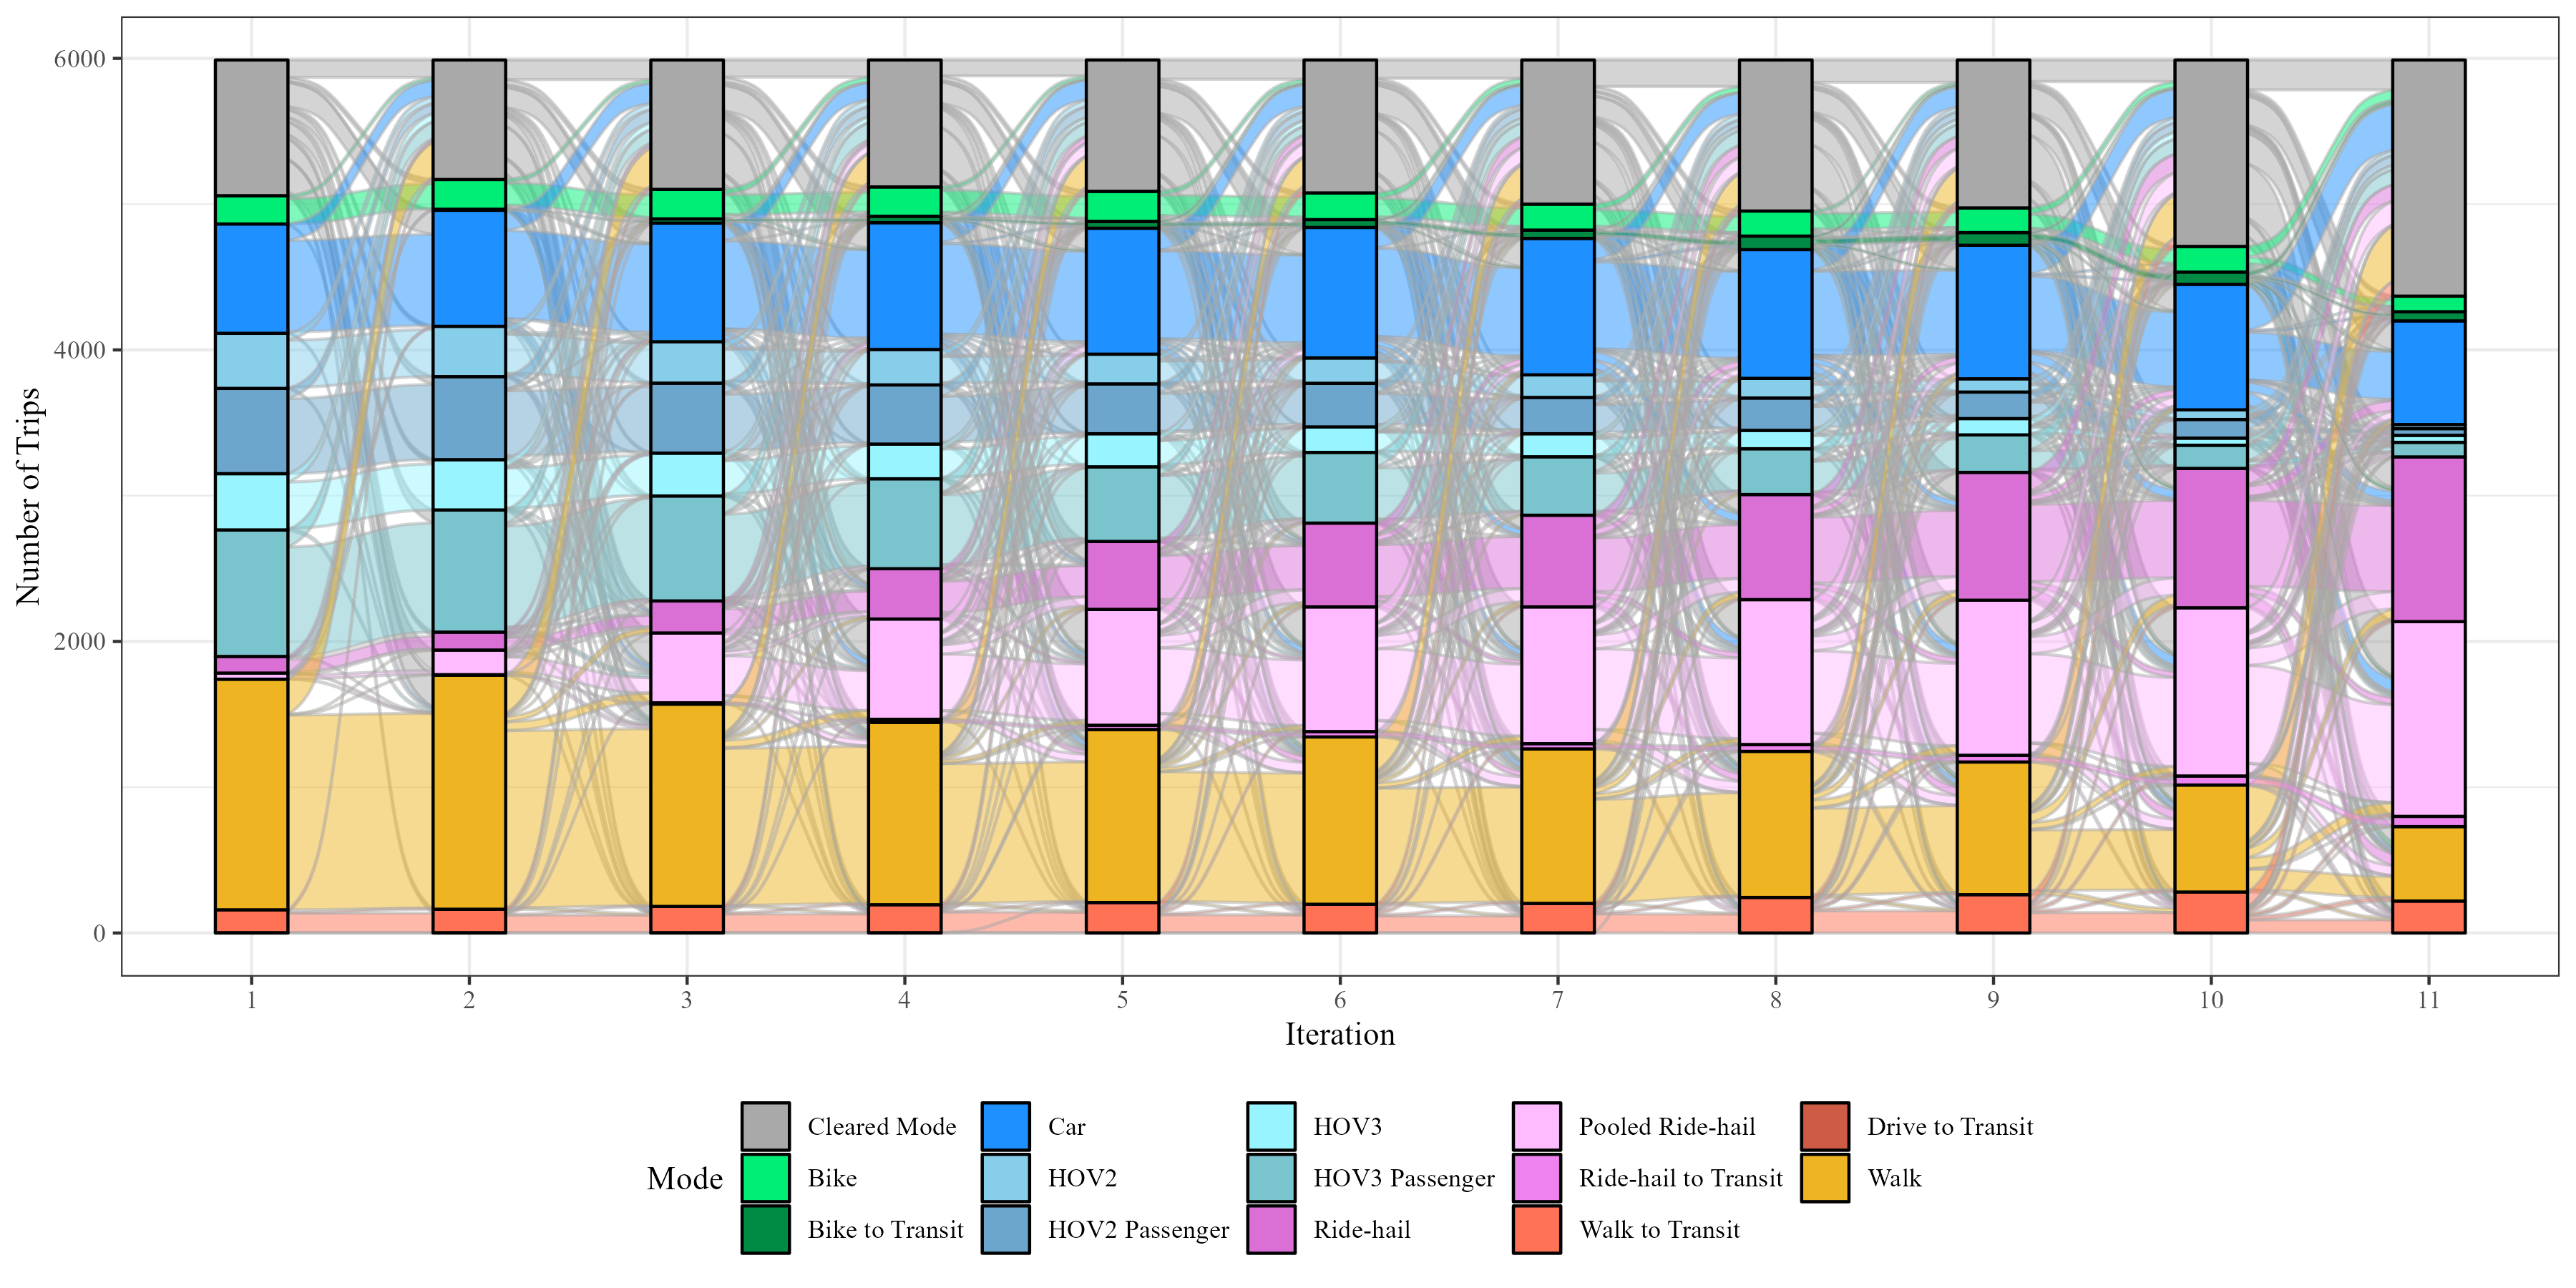
\includegraphics{planshifts.png}
\caption{The entire selection process of agents who use ride hail on the final iteration.}
\label{fig:sankey}
\end{figure}

\end{landscape}

The second factor for why agents switch from car to ride-hailing is BEAM's complex car tracking algorithm, which keeps track of household and agent level vehicle allocation. For example, if a household owns one vehicle, then the vehicle is \emph{assigned} to the first agent to use it in their daily plan. This leaves the other household members to choose an alternate mode. BEAM's implementation of vehicular assignment prevents many agents from selecting a car mode, whereas ActivitySim may not prevent those same individuals from car usage.

In addition to BEAM's vehicle assignment algorithm, BEAM's trip based mode choice structure forces some car users to switch modes. Sometimes, agents will \emph{lose} their vehicle within the day when a pathway cannot be built. If an agent \emph{loses} their car, car is no longer a valid modal alternative for future trips. Figure \ref{fig:walkers} provides evidence for this statement. Figure \ref{fig:walkers} displays a graph of those agents who start their day using a mode other than walk, but end up switching to the walk mode by the end of the day. Notice how in each hour, walk increases as car decreases or remains constant. Hundreds of car type mode users are switching to walk modes instead of remaining with their vehicle. Figure \ref{fig:sankey} shows that many walk users shift to ride-hailing each iteration. Therefore, car users who shift to walk on one trip, may shift to ride-hailing on the next trip. This is true between corresponding iterations as well. Overall, the increase in ridership in the \emph{All} model can be partially explained for these three reasons.

\begin{figure}

{\centering 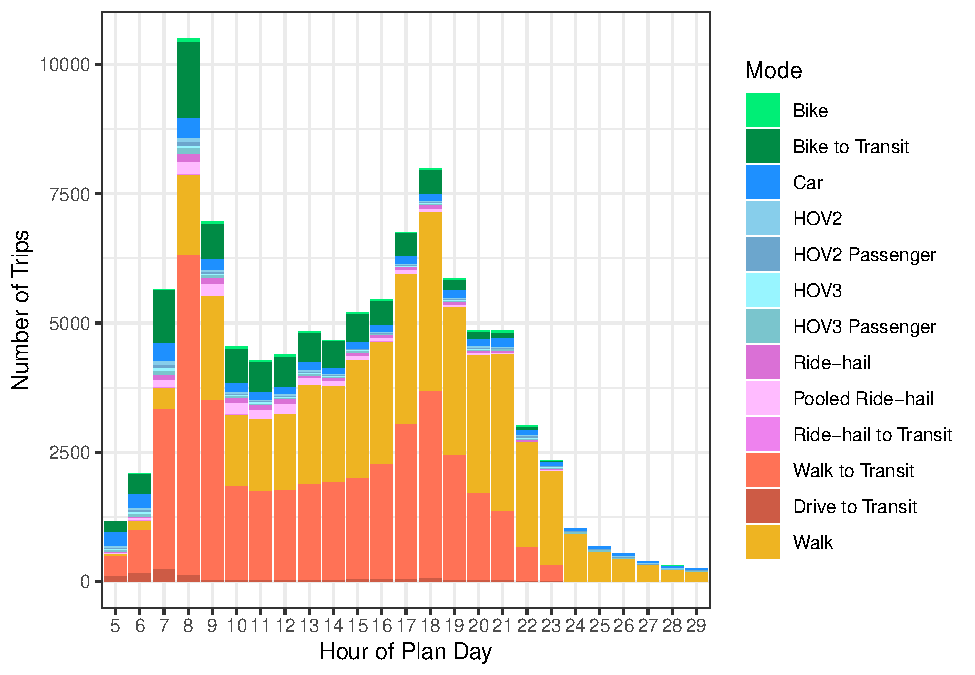
\includegraphics{thesis_files/figure-latex/walkers-1} 

}

\caption{Agents who switch to walk by time of day (AsimBeamAll:PPL).}\label{fig:walkers}
\end{figure}

\hypertarget{type2}{%
\subsection{Ridehail Mode Choice Model}\label{type2}}

Finally, the way the \emph{RideHail} BEAM mode choice model was constructed explains why their ridership and wait times were high. The \emph{RideHail} model only permits walk and transit users the option to switch to ride-hailing modes; car-type modes remained locked across each iteration. Whenever a ride-hailing path could be built, all walk modes were automatically given the option to choose ride hail or ride hail pooled and all transit modes were automatically given the option to choose ride hail transit. Although it made logical sense to lock all car-type modes (for reasons described in Section \ref{type3}), by giving ride hail options only to walk and transit users, ridership increased even more than in the \emph{All} scenario. The increase in ridership occurred because 1.) BEAM's adjusted code forced ride hail to be an option in almost all cases, and 2.) in most cases ride hail was calculated to be more attractive than walk or transit modes.

Table \ref{tab:timeutil} provides evidence in ride hail being an attractive mode choice alternative. Table \ref{tab:timeutil} displays the ride hail time utilization for each of the scenarios performed. The same ride hail fleet was used in each of the nine scenario, composed of 952 ride-hailing driver shifts. Ride hail time utilization was calculated as the sum of all the driver shift times divided by the sum of all passenger occupied ride-hailing travel time. The AsimRideHail scenario had the lowest ride hail time utilization, at only 4.046\%. Interestingly, the \emph{All} type scenarios ranged from 53.123\% to 62.459\% ride hail time utilization. This explains the higher wait times shown in Figure \ref{fig:waits}. Finally, by analyzing the ride hail time utilization for the \emph{RideHail} scenarios, we fully understand how attractive ride hail was. With 70.270\% to 73.777\% of ride hail time utilization present for the \emph{RideHail} scenarios, we see three fourths of each driver's shift was used to transport passengers. This explains the attractiveness of the choice, the extreme increase in ridership, and also the increased wait time for the \emph{RideHail} type scenarios.

\begin{table}

\caption{\label{tab:timeutil}Percent Ride Hail Time Utilization by Mode Choice Combination Scenario}
\centering
\begin{tabular}[t]{lr}
\toprule
ScenarioName & RideHailTimeUtilization\\
\midrule
AsimRideHail & 4.046\\
BeamRideHail:Path & 73.777\\
BeamRideHail:PPL & 70.270\\
AsimBeamRideHail:Path & 71.354\\
AsimBeamRideHail:PPL & 72.590\\
\addlinespace
BeamAll:Path & 62.459\\
BeamAll:PPL & 53.143\\
AsimBeamAll:Path & 58.739\\
AsimBeamAll:PPL & 53.123\\
\bottomrule
\end{tabular}
\end{table}

\hypertarget{summary-1}{%
\subsection{Summary}\label{summary-1}}

As seen by the explanation of the structure of the \emph{None}, \emph{All}, and \emph{RideHail} type scenarios, how BEAM's different mode choice structures were programmed affected ride-hailing ridership and wait time. Fortunately, section \ref{discussion} further describes the deeper meaning behind the ride hail, wait time, and mode choice structure results discovered in this section.

\hypertarget{discussion}{%
\chapter{Discussion}\label{discussion}}

The results presented in Section \ref{results} show that mode choice structure significantly affects forecasts of ride-hailing ridership and service capabilities. Slight changes to which mode choice alternatives are available for choice as well as which mode choice utility function is used impacts ridership and level of service greatly. In addition, the programming of the internal multi-agent simulation choice structure has a huge effect on results. The more advanced vehicular assignment model of a multi-agent simulation may be needed for more realistic modeled service behavior, but its increased complexity may cause irrational results. In our research the multi-agent simulation had a tendency to overstate the demand interest of ride-hailing vehicles, whereas the activity-based model did not. This was especially true when mode choice innovation was turned on and available to all walk and transit users. However, the \emph{All} model, described in Section \ref{meth-scenarios}, produced results closest to those predicted by the activity-based model (although still slightly overstated). This suggests that when the model structures of an activity-based model and a multi-agent simulation are aligned with similar utility equations and modal alternatives, optimal ride-hailing ridership and service capabilities can be produced.

The results also suggest that whether or not ride-hailing exists in the multi-agent simulation's input plans does not make a significant difference to total ride-hailing ridership or wait times. However, the purpose of using an activity-based model was to assign initial ride-hailing choices to the correct agents at the correct moments of their day. Therefore, although the estimation of service capabilities remained constant within the multi-agent simulation, the activity-based model had a background affect on making ride-hailing choices more realistic. We suggest that when the multi-agent simulation takes full control of estimating ride-hailing service capabilities, while the activity-based model determines who and when uses ride-hailing vehicles, optimal forecasts for ridership and level of service can be obtained. Unfortunately however, the estimations made by the multi-agent simulation in our research overpowered the estimations made by the activity-based model in most cases. Therefore, we believe a feedback loop between the activity-based model and the multi-agent simulation is needed to strengthen the forecasting power of ridehailing statistics.

\hypertarget{further-research}{%
\section{Further Research}\label{further-research}}

The results suggest the need for a feedback loop between an activity-based model and multi-agent simulation. We suggest an iterative process where the ride-hailing travel and wait times of the multi-agent simulation are inputted back into the activity-based model and the recalculated activity-based model ridership and usage values are inputted back into the multi-agent simulation. This process would continue, working off of each other, until the desired equilibrium and optimization of the ride-hailing system is achieved. Building upon the consistent mode choice model system designed in this research, this iterative process could establish more realistic and reliable ride-hailing ridership and level of service forecasts.

\hypertarget{limitations}{%
\chapter{Limitations}\label{limitations}}

Various components of the multi-agent simulation, BEAM, were not perfected. First, the mode choice coefficients in BEAM were not calibrated to exact regional values, and did not represent a completely accurate total modal distribution. This was left alone, however, as our primary research focus was to compare the effects of different mode choice structures and not predict accurate forecasts. In addition, some limitations existed within the BEAM software because BEAM was in development throughout the life of this project. One example is that activity plans remained constant across each iteration. Similarly, BEAM is not a tour based model whereas ActivitySim is. The BEAM developers also let us know that the plans files used to create Figure \ref{fig:sankey} were not a perfect representation of the mode choices chosen each iteration. These plans files did however give a sufficiently good idea of what was happening behind the scenes. The mode choice models we developed within BEAM also included a few limitations. The \emph{All} structure had various car-matching difficulties as well as path-building difficulties. The \emph{RideHail} structure gave the ride hail alternative to all individuals instead of only those who had undergone across day replanning.

The two biggest limitations with the input files related to the driver fleet and the network file. The driver fleet was developed by a fellow research student from another university, and the student did not factor in university and school location when statistically modeling the start location of each ride hail vehicle. Second, the network file we used only included main roadways, because it was too difficult to develop a reliable all streets network from the resources available. The last significant limitation of the research was that the results were from the 12th iteration of a 15\% scenario size. Due to our limited resources with computing power, larger scenarios and more iterations was too computationally heavy for our computers.

\hypertarget{conclusions}{%
\chapter{Conclusions}\label{conclusions}}

The advent of on-demand transport modes such as ride-hailing and microtransit has challenged forecasters with finding the best methodology to capturing behavior and estimating service capabilities. Ride-hailing and other novel modes have been forecasted with an array of different approaches like spatial analysis, activity-based models, and multi-agent simulation. Some professional disagreement exists as to which methodological approach should be used to best understand the availability and services capabilities of on-demand sevices. In particular, some question surrounds how successful a paired activity-based model and multi-agent simulation would fare in practice. By using the daily activity plans generated by ActivitySim, an activity-based model, as inputs to BEAM, a multi-agent simulation tool, we constructed nine different model combinations where the choice of ride-hailing varied between ActivitySim and BEAM. We also adjusted the mode choice utility equation between each model combination. By analyzing the ride-hailing ridership and level of service between each methodological combination, we found a promising approach to best forecaste ride-haling services. In our research the multi-agent simulation had a tendency to overestimate ride-hailing ridership, while estimating realistic level of service forecasts. As a result, we believe there is an opportunity to implement a feedback loop between an activity-based model and multi-agent simulation to create realistic and useful ride-hailing level of service and usage estimates.

Overall, accurately predicting the behavior and service capabilities of on-demand services is the key to a sustainable future. Ride-hailing and other novel modes are central to clean air, organized cities, and the effective movement of people. By accurately predicting the usage of ride-hailing and mictrotransit vehicles, we can help improve our cities and our lives. Overall, we can directly change the course of our future by how we estimate ride-hailing and other travel behavior, and so, should we not estimate it with the best approaches available? This research along with future research will help in these efforts to accurately predict the ever changing behavior and capabilities of transportation itself.

\hypertarget{appendix-a}{%
\chapter{Appendix A}\label{appendix-a}}

\hypertarget{apexA}{%
\section{Additions to the BEAM Mode Choice Model}\label{apexA}}

In order to use BEAM in conjunction with ActivitySim its mode choice model was updated to be more consistent with ActivitySim's mode choice model. More specifically, three changes were made to the choice structure:

\begin{enumerate}
\def\labelenumi{\arabic{enumi}.}
\tightlist
\item
  Adding a Tour Purpose Attribute
\item
  Adding Person, Path, and Location Attributes to the Utility Equation
\item
  Adding New Modal Alternatives
\end{enumerate}

First, we added a tour purpose attribute at the trip level, to be used when making trip-based modal decisions. ActivitySim's default utility parameters are segmented by tour purpose, auto ownership, and mode; therefore, it was essential to add a tour purpose level attribute to calculate the mode choice utility similar to ActivitySim.

Second, we added multiple person, path, and location related attributes to use in the mode choice utility equations. More specifically, we changed the BEAM utility equation to use Equation \eqref{eq:all} to calculate modal utility instead of Equation \eqref{eq:beam}. This was done by gathering path and location variables from the BEAM router and person level variables from the input files. ASCs were copied directly from the MTC ActivitySim example, and then calibrated later on. Overall, we created one input file which housed all path, person, and location type parameters on a tour purpose, auto ownership, and modal level.

Adding new modal alternatives was the last major adjustment we made to the BEAM software. The most important difference between the ActivitySim modal options and the BEAM modal options is the inclusion of carpooling vehicles (HOV2 and HOV3). HOV2 means High Occupancy Vehicle with 1 passenger (2 people in the vehicle) and HOV3 means High Occupancy Vehicle with 2 or more passengers (at least 3 people in the vehicle). We adjusted the BEAM software to include HOV2 and HOV3 type modes, including a distinction between drivers and passengers of those vehicles. Within the code, HOV2 and HOV3 modes were provided as modal options by transforming an existing car option into an HOV option. This allowed car travel statistics to be transferred over to the carpooling modes, which were essential to calculating the utility.

To understand the complexity of the new mode choice model in BEAM, two pseudocode algorithms are provided. Algorithm 1 describes the process behind determining the mode choice alternatives for each agent. This process occurs for every agent for every trip. Two procedures are presented within the first algorithm. The first procedure is called DetermineHOVAlternatives. In this procedure the HOV alternatives are created from already existing options created by the R5 router (Conveyal, 2022). (The R5 routing engine helps BEAM accomplish multi-modal routing). Basically if the R5 routing engine finds an existing car option, then both HOV2 and HOV3 options are provided for choice options as well. However, if the router doesn't generate any car pathways, then passenger HOV options are provided. Passenger HOV modes, called HOV\_TELEPORT, are completed by teleporting agents from origin to destination. The second procedure within Algorithm 1 describes the process behind determining the final modal alternatives. It states that if the current mode is already chosen, then no additional mode choice selection is needed. However, if no mode is currently chosen for the trip, the router, ride-hailing, and HOV alternatives are combined and presented as the final alternatives to choose from.

\begin{algorithm} [tph]
\caption{Algorithm for Determining Mode Choice Alternatives in BEAM}
\begin{algorithmic}[1]
\Require
\State $i : origin$
\State $j : destination$
\State $n: agent$
\State $N: population$
\State $t : trip $
\State $P : plan$
\State $\vec{R}(i,j) : Router\: alternatives$
\State $\vec{RH}(i,j) : Ridehail\:alternatives$
\State $\vec{H}(i,j) : HOV\:alternatives$
\State $\vec{M}(i,j) : Final\:modal\:alternatives$
\State $C : Current\:Mode$
\State $I : Trip\:Index$
\vspace{4pt}\hrule\vspace{5pt}

\State $\vec{R} \equiv \vec{R}(i,j)$
\State $\vec{RH} \equiv \vec{RH}(i,j)$
\State $\vec{H} \equiv \vec{H}(i,j)$
\State $\vec{M} \equiv \vec{M}(i,j)$
\For {$n \in N$}
\For {$t \in P$}

\Procedure {DetermineHOVAlternatives}{$\vec{R}$, $C$}
\If {$C=None$}
  \If {$\vec{R} \ni CAR$}
    \State $\vec{H} \gets (HOV2,HOV3)$
  \ElsIf {$\vec{R} \ni HOV2$}
    \State $\vec{H} \gets (HOV3)$
  \ElsIf {$\vec{R} \ni HOV3$}
    \State $\vec{H} \gets (HOV2)$
  \ElsIf {$\vec{R} \ni WALK$}
    \State $\vec{H} \gets (HOV2\_TELEPORT, HOV3\_TELEPORT)$
  \EndIf
\Else
  \State $\vec{H} \gets None$
\EndIf
\EndProcedure
\Statex
\algstore{myalg}
\end{algorithmic}
\end{algorithm}

\addtocounter{algorithm}{-1}
\begin{algorithm}
\caption{continued}
\begin{algorithmic} [1]
\algrestore{myalg}
\Procedure {DetermineModalAlternatives}{$\vec{R}$, $\vec{RH}$, $\vec{H}$, $C$, $I$}
\If {$C = DRIVE\_TRANSIT \lor BIKE\_TRANSIT$}
  \If {$I = 0$}
    \If {$C = DRIVE\_TRANSIT$}
      \State $\vec{M} \gets (DRIVE\_TRANSIT)$
    \Else
      \State $\vec{M} \gets (BIKE\_TRANSIT)$
    \EndIf  
  \Else
    \State $\vec{M} \gets (WALK\_TRANSIT, RIDEHAIL\_TRANSIT)$
  \EndIf
\ElsIf {$C = WALK\_TRANSIT \lor RIDEHAIL\_TRANSIT$}  
  \If {$C = WALK\_TRANSIT$}
    \State $\vec{M} \gets (WALK\_TRANSIT)$
  \Else
    \State $\vec{M} \gets (RIDEHAIL\_TRANSIT)$
  \EndIf
\ElsIf {$C = HOV2\_TELEPORT \lor HOV3\_TELEPORT$}  
  \If {$C = HOV2\_TELEPORT$}
    \State $\vec{M} \gets (HOV2\_TELEPORT)$
  \Else
    \State $\vec{M} \gets (HOV3\_TELEPORT)$
  \EndIf
\ElsIf {$C = CAR$}
  \State $\vec{M} \gets (CAR)$
\Else
  \State $\vec{M} \gets \vec{R} + \vec{RH} + \vec{H}$  
\EndIf  
\EndProcedure
\EndFor
\EndFor
\Statex
\end{algorithmic}
\end{algorithm}

Algorithm 2 describes the mathematical process within BEAM for how one modal alternative is selected among all the mode choice options. By calculating the probability of choosing each modal alternative, and sampling those probabilities, a final mode choice is selected and used.

\begin{algorithm}
\caption{Algorithm for Selecting Modal Alternative in BEAM}
\begin{algorithmic}[1]
\Require
\State $i : origin$
\State $j : destination$
\State $n: agent$
\State $N: population$
\State $t : trip $
\State $P : plan$
\State $\vec{A}: attributes\:of\:agent$
\State $a: attribute\:value$
\State $\vec{M}(i,j) : Modal\:alternatives$
\State $m : alternative \in M(i,j)$
\State $\vec{U}(\vec{M}(i,j),\vec{A}):Utilities\:for\:alternatives$
\State $u: utility \in \vec{U}(\vec{M}(i,j),\vec{A})$
\State $\vec{c}: attribute\:coefficients$
\State $\mathds{P}: probability$
\State $Mode: chosen\:mode\:for\:agent\:(n)\:on\:trip\:(t)$
\State $f(\vec{X}):$
This function takes a vector of modes and  their probabilities of being chosen. With those probabilities it builds them into a cumulative distribution function, generates a random number and then drops the mode with the closest probability. This process continues until only one mode is left.
\vspace{4pt}\hrule\vspace{5pt}

\State $\vec{M} \equiv \vec{M}(i,j)$
\State $\vec{U} \equiv \vec{U}(\vec{M},\vec{A})$
\For {$n \in N$}
\For {$t \in P$}\Procedure {DetermineModalAlternative}{$\vec{M}$, $\vec{A}$, $\vec{c}$}
\For {$m \in \vec{M}$}
  \State $u \gets \sum_{a\in \vec{A}} a \times c_a$
  \State $\vec{U} += [m,u]$
\EndFor
\State $S \gets \sum_{u\in \vec{U}}e^u$
\For {$u \in \vec{U}$}
    \State $\mathds{P}(u)\gets e^u / S$
    \State $\vec{B} +=[m, \mathds{P}(u)]$
\EndFor 

\State $Mode \gets f(\vec{B})$

\EndProcedure

\EndFor
\EndFor
\Statex
\end{algorithmic}
\end{algorithm}

\hypertarget{references}{%
\chapter*{References}\label{references}}
\addcontentsline{toc}{chapter}{References}

\hypertarget{refs}{}
\begin{CSLReferences}{1}{0}
\leavevmode\vadjust pre{\hypertarget{ref-asim}{}}%
ActivitySim. (2021a). \emph{ActivitySim: An open platform for activity-based travel modeling} (Version 0.9.9.1) {[}Computer software{]}. \url{https://github.com/ActivitySim/activitysim.}

\leavevmode\vadjust pre{\hypertarget{ref-rsg21}{}}%
ActivitySim: An advanced activity-based travel demand model built by and for users. (2021b). In \emph{RSG}. \url{https://rsginc.com/activitysim-white-paper/\#advanced-activity-based-travel-demand-model}

\leavevmode\vadjust pre{\hypertarget{ref-agrc}{}}%
AGRC. (2021). \emph{Automated geographic reference center}. \url{https://gis.utah.gov/}

\leavevmode\vadjust pre{\hypertarget{ref-amblard15}{}}%
Amblard, F., Daudé, E., Gaudou, B., Grignard, A., Hutzler, G., Lang, C., Marilleau, N., Nicod, J.-M., Sheeren, D., \& Taillandier, P. (2015). Introduction to NetLogo. In \emph{Agent-based spatial simulation with netlogo} (pp. 75--123). Elsevier.

\leavevmode\vadjust pre{\hypertarget{ref-bazghandi12}{}}%
Bazghandi, A. (2012). Techniques, advantages and problems of agent based modeling for traffic simulation. \emph{International Journal of Computer Science Issues (IJCSI)}, \emph{9}(1), 115.

\leavevmode\vadjust pre{\hypertarget{ref-beam}{}}%
BEAM. (2022). \emph{Behavior, energy, autonomy, and mobility}. Lawrence Berkeley National Laboratory the UC Berkeley Institute for Transportation Studies. \url{https://beam.readthedocs.io/en/develop/users.html}

\leavevmode\vadjust pre{\hypertarget{ref-becker20}{}}%
Becker, H., Balac, M., Ciari, F., \& Axhausen, K. W. (2020). Assessing the welfare impacts of shared mobility and mobility as a service (MaaS). \emph{Transportation Research Part A: Policy and Practice}, \emph{131}, 228--243.

\leavevmode\vadjust pre{\hypertarget{ref-biehl19}{}}%
Biehl, A., Ermagun, A., \& Stathopoulos, A. (2019). Utilizing multi-stage behavior change theory to model the process of bike share adoption. \emph{Transport Policy}, \emph{77}, 30--45.

\leavevmode\vadjust pre{\hypertarget{ref-bowman98}{}}%
Bowman, J. L. (1998). \emph{The day activity schedule approach to travel demand analysis} {[}PhD thesis{]}. Massachusetts Institute of Technology.

\leavevmode\vadjust pre{\hypertarget{ref-nchrp}{}}%
Cambridge Systematics, Inc., Vanasse Hangen Brustlin, Inc., Corporation, G., Bhat, C. R., Shapiro Transportation Consulting, L., \& Martin/Alexiou/Bryson, P. (2012). Travel demand forecasting: Parameters and techniques. In \emph{NCHRP report 716} (pp. 55--60). Transportation Research Board.

\leavevmode\vadjust pre{\hypertarget{ref-chen21}{}}%
Chen, L., Thakuriah, P. V., \& Ampountolas, K. (2021). Short-term prediction of demand for ride-hailing services: A deep learning approach. \emph{Journal of Big Data Analytics in Transportation}, \emph{3}(2), 175--195.

\leavevmode\vadjust pre{\hypertarget{ref-cho22}{}}%
Cho, S.-H., \& Shin, D. (2022). Estimation of route choice behaviors of bike-sharing users as first-and last-mile trips for introduction of mobility-as-a-service (MaaS). \emph{KSCE Journal of Civil Engineering}, 1--12.

\leavevmode\vadjust pre{\hypertarget{ref-ciari16}{}}%
Ciari, F., Balac, M., \& Axhausen, K. W. (2016). Modeling carsharing with the agent-based simulation MATSim: State of the art, applications, and future developments. \emph{Transportation Research Record}, \emph{2564}(1), 14--20.

\leavevmode\vadjust pre{\hypertarget{ref-r5}{}}%
Conveyal. (2022). \emph{R5: Rapid realistic routing on real-world and reimagined networks}. \url{https://github.com/conveyal/r5}

\leavevmode\vadjust pre{\hypertarget{ref-correa17}{}}%
Correa, D., Xie, K., \& Ozbay, K. (2017). Exploring the taxi and uber demand in new york city: An empirical analysis and spatial modeling. \emph{96th Annual Meeting of the Transportation Research Board, Washington, DC}.

\leavevmode\vadjust pre{\hypertarget{ref-dean21}{}}%
Dean, M. D., \& Kockelman, K. M. (2021). Spatial variation in shared ride-hail trip demand and factors contributing to sharing: Lessons from chicago. \emph{Journal of Transport Geography}, \emph{91}, 102944.

\leavevmode\vadjust pre{\hypertarget{ref-dong20}{}}%
Dong, X. (2020). Trade uber for the bus? \emph{Journal of the American Planning Association}, \emph{86}(2), 222--235.

\leavevmode\vadjust pre{\hypertarget{ref-dong18}{}}%
Dong, Y., Wang, S., Li, L., \& Zhang, Z. (2018). An empirical study on travel patterns of internet based ride-sharing. \emph{Transportation Research Part C: Emerging Technologies}, \emph{86}, 1--22.

\leavevmode\vadjust pre{\hypertarget{ref-gomes21}{}}%
Gomes, V. A., CALDAS, M., \& Pitombo, C. S. (2021). An investigation of trip-chaining behaviour based on activity participation, socioeconomic variables and aggregated characteristics of modal alternatives. \emph{Revista Transportes}, \emph{29}(1), 21--41.

\leavevmode\vadjust pre{\hypertarget{ref-hasnine21}{}}%
Hasnine, M. S., \& Nurul Habib, K. (2021). Tour-based mode choice modelling as the core of an activity-based travel demand modelling framework: A review of state-of-the-art. \emph{Transport Reviews}, \emph{41}(1), 5--26.

\leavevmode\vadjust pre{\hypertarget{ref-horl19}{}}%
Hörl, S., Balać, M., \& Axhausen, K. W. (2019). Pairing discrete mode choice models and agent-based transport simulation with MATSim. \emph{2019 TRB Annual Meeting Online}, 19--02409.

\leavevmode\vadjust pre{\hypertarget{ref-horl19b}{}}%
Hörl, S., Ruch, C., Becker, F., Frazzoli, E., \& Axhausen, K. W. (2019). Fleet operational policies for automated mobility: A simulation assessment for zurich. \emph{Transportation Research Part C: Emerging Technologies}, \emph{102}, 20--31.

\leavevmode\vadjust pre{\hypertarget{ref-hosseinzadeh21}{}}%
Hosseinzadeh, A., Algomaiah, M., Kluger, R., \& Li, Z. (2021). Spatial analysis of shared e-scooter trips. \emph{Journal of Transport Geography}, \emph{92}, 103016.

\leavevmode\vadjust pre{\hypertarget{ref-hyland18}{}}%
Hyland, M., Hong, Z., Farias Pinto, H. K. R. de, \& Chen, Y. (2018). Hybrid cluster-regression approach to model bikeshare station usage. \emph{Transportation Research Part A: Policy and Practice}, \emph{115}, 71--89.

\leavevmode\vadjust pre{\hypertarget{ref-kamel19}{}}%
Kamel, J., Vosooghi, R., Puchinger, J., Ksontini, F., \& Sirin, G. (2019). Exploring the impact of user preferences on shared autonomous vehicle modal split: A multi-agent simulation approach. \emph{Transportation Research Procedia}, \emph{37}, 115--122.

\leavevmode\vadjust pre{\hypertarget{ref-kang21}{}}%
Kang, S., Mondal, A., Bhat, A. C., \& Bhat, C. R. (2021). Pooled versus private ride-hailing: A joint revealed and stated preference analysis recognizing psycho-social factors. \emph{Transportation Research Part C: Emerging Technologies}, \emph{124}, 102906.

\leavevmode\vadjust pre{\hypertarget{ref-knapen21}{}}%
Knapen, L., Adnan, M., Kochan, B., Bellemans, T., Tuin, M. van der, Zhou, H., \& Snelder, M. (2021). An activity based integrated approach to model impacts of parking, hubs and new mobility concepts. \emph{Procedia Computer Science}, \emph{184}, 428--437.

\leavevmode\vadjust pre{\hypertarget{ref-nate}{}}%
Lant, N. J. (2021). \emph{Estimation and simulation of daily activity patterns for individuals using wheelchairs} {[}PhD thesis{]}. Brigham Young University.

\leavevmode\vadjust pre{\hypertarget{ref-leeb21}{}}%
Lee, H., Baek, K., Chung, J.-H., \& Kim, J. (2021). Factors affecting heterogeneity in willingness to use e-scooter sharing services. \emph{Transportation Research Part D: Transport and Environment}, \emph{92}, 102751.

\leavevmode\vadjust pre{\hypertarget{ref-lee21}{}}%
Lee, M., Chow, J. Y., Yoon, G., \& He, B. Y. (2021). Forecasting e-scooter substitution of direct and access trips by mode and distance. \emph{Transportation Research Part D: Transport and Environment}, \emph{96}, 102892.

\leavevmode\vadjust pre{\hypertarget{ref-li18}{}}%
Li, W., \& Kamargianni, M. (2018). Providing quantified evidence to policy makers for promoting bike-sharing in heavily air-polluted cities: A mode choice model and policy simulation for taiyuan-china. \emph{Transportation Research Part A: Policy and Practice}, \emph{111}, 277--291.

\leavevmode\vadjust pre{\hypertarget{ref-li22}{}}%
Li, W., Shalaby, A., \& Habib, K. N. (2022). Exploring the correlation between ride-hailing and multimodal transit ridership in toronto. \emph{Transportation}, \emph{49}(3), 765--789.

\leavevmode\vadjust pre{\hypertarget{ref-li20}{}}%
Li, Y., Liu, Y., \& Xie, J. (2020). A path-based equilibrium model for ridesharing matching. \emph{Transportation Research Part B: Methodological}, \emph{138}, 373--405.

\leavevmode\vadjust pre{\hypertarget{ref-macfarlane21}{}}%
Macfarlane, G. S., Lant, N. J., et al. (2021). \emph{Estimation and simulation of daily activity patterns for individuals using wheelchairs}. Utah. Dept. of Transportation. Division of Research.

\leavevmode\vadjust pre{\hypertarget{ref-mahmoudi21}{}}%
Mahmoudi, M., Tong, L. (Carol), Garikapati, V. M., Pendyala, R. M., \& Zhou, X. (2021). How many trip requests could we support? An activity-travel based vehicle scheduling approach. \emph{Transportation Research Part C: Emerging Technologies}, \emph{128}. https://doi.org/\url{https://doi.org/10.1016/j.trc.2021.103222}

\leavevmode\vadjust pre{\hypertarget{ref-marquet20}{}}%
Marquet, O. (2020). Spatial distribution of ride-hailing trip demand and its association with walkability and neighborhood characteristics. \emph{Cities}, \emph{106}, 102926.

\leavevmode\vadjust pre{\hypertarget{ref-moeckel20}{}}%
Moeckel, R., Kuehnel, N., Llorca, C., Moreno, A. T., \& Rayaprolu, H. (2020). Agent-based simulation to improve policy sensitivity of trip-based models. \emph{Journal of Advanced Transportation}, \emph{2020}.

\leavevmode\vadjust pre{\hypertarget{ref-mtc12}{}}%
MTC. (2012). In \emph{Travel Model Development: Calibration and Validation Technical Report}. Metropolitan Transportation Commission with Parsons Brinckerhoff, Inc.

\leavevmode\vadjust pre{\hypertarget{ref-muhammad19}{}}%
Muhammad, H., IQBAL, A., ADNAN, M., KOCHAN, B., BELLEMANS, T., \& JANSSENS, D. (2019). \emph{Incorporating MaaS concept into an operational activity-based modelling platform}.

\leavevmode\vadjust pre{\hypertarget{ref-nayak22}{}}%
Nayak, S., \& Pandit, D. (2022). Activity-based model: Requisite for a new travel demand forecasting approach for india. \emph{Proceedings of the Fifth International Conference of Transportation Research Group of India}, 109--121.

\leavevmode\vadjust pre{\hypertarget{ref-nguyen22}{}}%
Nguyen, T. K., Hoang, N. H., \& Vu, H. L. (2022). A unified activity-based framework for one-way car-sharing services in multi-modal transportation networks. \emph{Transportation Research Part E: Logistics and Transportation Review}, \emph{157}, 102551.

\leavevmode\vadjust pre{\hypertarget{ref-philip13}{}}%
Philip, M., Sreelatha, T., \& George, S. (2013). Activity based travel behavioural study and mode choice modelling. \emph{Int J Innov Res Sci Eng Technol}, \emph{2}(1), 181--190.

\leavevmode\vadjust pre{\hypertarget{ref-popsim}{}}%
PopulationSim. (2021). \emph{An open platform for population synthesis} (Version 0.5) {[}Computer software{]}. \url{https://activitysim.github.io/populationsim/}

\leavevmode\vadjust pre{\hypertarget{ref-rafiq22}{}}%
Rafiq, R., \& McNally, M. G. (2022). An exploratory analysis of alternative travel behaviors of ride-hailing users. \emph{Transportation}, 1--35.

\leavevmode\vadjust pre{\hypertarget{ref-rsg16}{}}%
RSG. (2016). In \emph{Pricing and Travel Time Reliability Enhancements in the SANDAG Activity-Based Travel Model: Final Report}.

\leavevmode\vadjust pre{\hypertarget{ref-sanchez19}{}}%
Sánchez, P., Pato, D., Martín, G., et al. (2019). \emph{CTRANSPORT: Multi-agent-based simulation}.

\leavevmode\vadjust pre{\hypertarget{ref-shimizu13}{}}%
Shimizu, S., Akai, K., \& Nishino, N. (2013). Modeling and multi-agent simulation of bicycle sharing. \emph{International Conference on Serviceology}, 39--46.

\leavevmode\vadjust pre{\hypertarget{ref-siebers08}{}}%
Siebers, P.-O., \& Aickelin, U. (2008). Introduction to multi-agent simulation. In \emph{Encyclopedia of decision making and decision support technologies} (pp. 554--564). IGI Global.

\leavevmode\vadjust pre{\hypertarget{ref-song19}{}}%
Song, M., Zhang, Y., Shen, Z. M., Li, M., \& Dong, Z. (2019). Mode shift from car to bike shared: A travel-mode choice model. In \emph{CICTP 2019} (pp. 2398--2410).

\leavevmode\vadjust pre{\hypertarget{ref-tuli21}{}}%
Tuli, F. M., Mitra, S., \& Crews, M. B. (2021). Factors influencing the usage of shared e-scooters in chicago. \emph{Transportation Research Part A: Policy and Practice}, \emph{154}, 164--185.

\leavevmode\vadjust pre{\hypertarget{ref-utahstate}{}}%
UDOT. (2021). \emph{Utah state travel demand model}. Utah Department of Transportation.

\leavevmode\vadjust pre{\hypertarget{ref-welch20}{}}%
Welch, T. F., Gehrke, S. R., \& Widita, A. (2020). Shared-use mobility competition: A trip-level analysis of taxi, bikeshare, and transit mode choice in washington, DC. \emph{Transportmetrica A: Transport Science}, \emph{16}(1), 43--55.

\leavevmode\vadjust pre{\hypertarget{ref-wfrc}{}}%
WFRC. (2019). \emph{Wasatch front travel demand model} (Version v8.3.1) {[}Computer software{]}. Wasatch Front Regional Council. \url{https://wfrc.org/programs/models-forecasting/}

\leavevmode\vadjust pre{\hypertarget{ref-xu19}{}}%
Xu, X., Mahmassani, H. S., \& Chen, Y. (2019). Privately owned autonomous vehicle optimization model development and integration with activity-based modeling and dynamic traffic assignment framework. \emph{Transportation Research Record}, \emph{2673}(10), 683--695.

\leavevmode\vadjust pre{\hypertarget{ref-zhang21}{}}%
Zhang, W., Buehler, R., Broaddus, A., \& Sweeney, T. (2021). What type of infrastructures do e-scooter riders prefer? A route choice model. \emph{Transportation Research Part D: Transport and Environment}, \emph{94}, 102761.

\leavevmode\vadjust pre{\hypertarget{ref-zhou19}{}}%
Zhou, X., Wang, M., \& Li, D. (2019). Bike-sharing or taxi? Modeling the choices of travel mode in chicago using machine learning. \emph{Journal of Transport Geography}, \emph{79}, 102479.

\leavevmode\vadjust pre{\hypertarget{ref-zuniga22}{}}%
Zuniga-Garcia, N., Tec, M., Scott, J. G., \& Machemehl, R. B. (2022). Evaluation of e-scooters as transit last-mile solution. \emph{Transportation Research Part C: Emerging Technologies}, \emph{139}, 103660.

\leavevmode\vadjust pre{\hypertarget{ref-zwick21}{}}%
Zwick, F., Kuehnel, N., Moeckel, R., \& Axhausen, K. W. (2021). Agent-based simulation of city-wide autonomous ride-pooling and the impact on traffic noise. \emph{Transportation Research Part D: Transport and Environment}, \emph{90}, 102673.

\end{CSLReferences}

%%%%%%%%%%%%%%%%%%%%%%%%
% --- Bibliography --- %
%%%%%%%%%%%%%%%%%%%%%%%%
% printed automatically with CSL
%
%%%%%%%%%%%%%%%%%%%%%
% --- Appendices --- %
%%%%%%%%%%%%%%%%%%%%%


\end{document}
